\documentclass[11pt,fleqn]{article}
\usepackage[margin=1in,top=1in,bottom=1in]{geometry}
\usepackage{mathtools}
\usepackage{longtable}
\usepackage{enumitem}
\usepackage{hyperref}
\usepackage[dvips]{graphics}
\usepackage[table]{xcolor}
\usepackage{amssymb}
\usepackage{float}
\usepackage{booktabs}

\usepackage[normalem]{ulem}

\usepackage{multicol}
\usepackage{txfonts}
\usepackage{amsfonts}
\usepackage{natbib}
\usepackage{gb4e}
\usepackage[all]{xy}
\usepackage{rotating}
\usepackage{tipa}
\usepackage{multirow}
\usepackage{authblk}
\usepackage{url}

\def\bad{{\leavevmode\llap{*}}}
\def\marginal{{\leavevmode\llap{?}}}
\def\verymarginal{{\leavevmode\llap{??}}}
\def\swmarginal{{\leavevmode\llap{4}}}
\def\infelic{{\leavevmode\llap{\#}}}

\setlength{\parindent}{.3in}
\setlength{\parskip}{0ex}

%\renewcommand{\baselinestretch}{1.2}

\newcommand{\yi}{\'{\symbol{16}}}
\newcommand{\nasi}{\~{\symbol{16}}}
\newcommand{\hina}{h\nasi na}
\newcommand{\ina}{\nasi na}

\newcommand{\foc}{$_{\mbox{\small F}}$}

\hyphenation{par-ti-ci-pa-tion}

\setlength{\bibhang}{0.5in}
\setlength{\bibsep}{0mm}
\bibpunct[:]{(}{)}{,}{a}{}{,}

\newcommand{\6}{\mbox{$[\hspace*{-.6mm}[$}} 
\newcommand{\9}{\mbox{$]\hspace*{-.6mm}]$}}
\newcommand{\sem}[2]{\6#1\9$^{#2}$}
\renewcommand{\ni}{\~{\i}}

\newcommand{\citepos}[1]{\citeauthor{#1}'s \citeyear{#1}}
\newcommand{\citeposs}[1]{\citeauthor{#1}'s}
\newcommand{\citetpos}[1]{\citeauthor{#1}'s (\citeyear{#1})}


%From Mandy conversation:
%- add sentence on p.15 that this meaning is not the final version
%- section 3.2: more nuanced discussion about whether previous analyses assume that prejacent is entailed
%- unacceptable because contradictory: no imaginable circumstance where not-prejacent but S
%- 23c is odd for mandy, perhaps need footnote
%- "will" is part of the prejacent for judging the entailments in 23
%- Mandy wants "enough" even in positive example 23b so "enough" has nothing to do with negation or projection


\title{Evaluative adjective sentences: \\ A question-based analysis of projection\thanks{For helpful comments and critical feedback, we thank David Beaver, Ashwini Deo, Lauri Karttunen, Stanley Peters, Craige Roberts,
Stephanie Solt and the audiences at the following venues: the 6th meeting of the DFG Network
{\em Questions in Discourse} at the University of G\"ottingen, 
the University of Stuttgart, the 16th Sklarska Poreba workshop, the
Redrawing Pragmasemantic Borders workshop at the University of
Groningen, the University of Cologne, Oxford University, the University of T\"ubingen,  the University of G\"ottingen, the {\em
Experimental Pragmatics} 2015 conference in Chicago, The Ohio State
University and Cornell University. We thank Willy Cheung for his assistance with the corpus study. We gratefully acknowledge
financial support from the {\em National Science Foundation} (grants
BCS-0952571 and BCS-1452674), the Alexander von Humboldt Foundation and the Ohio State
University College of Arts and Sciences Targeted Investment in
Excellence initiative.}}

\author[$\circ$]{Judith Tonhauser}
\author[$\bullet$]{Judith Degen}
\author[$\circ$]{Marie-Catherine de Marneffe}
\author[$\star$]{Mandy Simons}

\affil[$\circ$]{The Ohio State University}
\affil[$\bullet$]{Stanford University}
\affil[$\star$]{Carnegie Mellon University}

\renewcommand\Authands{ and }

\newcommand{\jt}[1]{\textbf{\color{blue}JT: #1}}
\newcommand{\jd}[1]{\textbf{\color{green}[jd: #1]}} 


\begin{document}

%\tableofcontents
%\newpage

\maketitle

\begin{abstract}



Evaluative adjective sentences are standardly analyzed as presupposing the prejacent: for instance, {\em Kim wasn't smart to
watch the movie} is taken to presuppose that Kim watched the movie
(e.g., \citealt{norrick78,barker02,oshima09b,kertz2010}). This paper argues against an analysis of the prejacent as a lexically-specified presupposition and proposes instead that the projectivity of the prejacent depends on the question addressed by the utterance of the evaluative adjective sentence (\citealt{beaver-clark08,best-question,brst-ar}). Evidence for the proposed analysis comes from a study of the projectivity of the prejacent in naturally occurring evaluative adjective sentences and two experiments that show that the at-issueness and projectivity of the prejacent are sensitive to the question addressed by the utterance of the evaluative adjective sentence. The proposed analysis is also compared with that of \citealt{karttunen-etal2014}, according to which evaluative adjective sentences are systematically ambiguous. 


\end{abstract}


\section{Introduction}\label{s1}

In an evaluative adjective sentence (EAS) like (\ref{f}), the
evaluative adjective {\em stupid} subcategorizes for a non-pleonastic subject noun
phrase ({\em Feynman}) and a {\em to-}infinitive ({\em to
dance on the table}); the subject of the predicate {\em be stupid} is the understood subject of the {\em to-}infinitive (e.g., \citealt{wilkinson70, norrick78,barker02,kertz2010}). Two contents of EASs that this paper is concerned with are the `prejacent' and the `evaluation': in (\ref{f}), the prejacent is that Feynman danced on the table and the evaluation is that 
Feynman dancing on the table was stupid.\footnote{This paper ignores the subject-related presuppositions discussed in \citealt{barker02}.}

\begin{exe} \ex\label{f} Feynman was stupid to dance on the table. \hfill (\citealt[18]{barker02})

\end{exe} 

EASs have traditionally been analyzed as presupposing the prejacent (e.g., \citealt{norrick78,barker02,oshima09b,kertz2010}). On such analyses,  evaluative adjectives like {\em stupid} lexically specify that the prejacent
must be entailed by or satisfied in the common ground of the interlocutors in
order for an EAS to be interpretable (e.g.,
\citealt{heim83,vds92}). Such analyses are motivated by and straightforwardly account for examples like those in (\ref{f2}a-d) in which the prejacent projects over entailment-canceling operators, i.e., negation in (\ref{f2}a), a polar question in (\ref{f2}b), the possibility adverb {\em perhaps} in (\ref{f2}c) and the antecedent of the conditional in (\ref{f2}d). That is, speakers who utter (\ref{f2}a-d) may be taken to be committed to the prejacent, that Feynman danced on the table, even though the evaluative adjective occurs under an entailment-canceling operator. The evaluation, on the other hand, that Feyman dancing on the table was stupid, is not projective content but denied in (\ref{f2}a), questioned in (\ref{f2}b), and merely considered a possibility in (\ref{f2}c) and (\ref{f2}d).

\begin{exe}

\ex\label{f2} 

\begin{xlist}

\ex Feynman wasn't stupid to dance on the table.

\ex Was Feynman stupid to dance on the table?

\ex Perhaps Feynman was stupid to dance on the table.

\ex If Feynman was stupid to dance on the table, then tell him. \hfill (\citealt[18f.]{barker02})

\end{xlist}
\end{exe}

Recently, \citet{karttunen-etal2014} provided naturally occurring examples that show that utterances of sentences in which the evaluative adjective is embedded under negation can receive interpretations according to which the prejacent
does not project, but is interpreted in the scope of negation. For instance, the speaker of (\ref{nat}a) is not committed to living close to their parents and instead communicates that they do not live close to their parents. Likewise, the speaker of (\ref{nat}b) is not committed to having stumbled through the junkyard in the dark but rather communicates that they did not stumble through the junkyard.

\begin{exe}
\ex\label{nat} \citealt[235]{karttunen-etal2014}
\begin{xlist}
\ex I wasn't fortunate to live extremely close to my Mom and Dad for most of my adult life. The closest was when I was in Denver and they were in Garden City, KS.

%\ex This is my first trip to Italy, so I was not \fbox{brave} to venture out alone.

\ex  Now I knew someone was in the junkyard and the cold wind was
carrying the cries. I wasn't stupid to go stumbling through the
junkyard in the dark and get hurt.

\end{xlist} \end{exe} 

We discuss below why such examples are problematic for analyses according to which the prejacent is a presupposition. But we first need to mention that even though all native speakers of American English appear to be able to retrieve the intended interpretations of examples like (\ref{nat}), a sizeable portion strongly prefers to realize such interpretations with variants that includes {\em enough}, as in {\em I wasn't stupid enough to go stumbling through the junkyard in the dark} for (\ref{nat}b); see also \citealt{karttunen2013} and \citealt{karttunen-etal2014} for this observation. Our goal in this paper is to analyze the interpretation of EASs and we assume that all native speakers of American English have access to both interpretations, that is, an interpretation according to which the prejacent projects, as in (\ref{f2}), and an interpretation according to which it doesn't project, as in (\ref{nat}). Evidence that examples in which the prejacent does not project are part of the productive language use of some native speakers of American English comes from the existence of naturally occurring examples like (\ref{nat}); further  such examples are presented in this paper. Additional evidence comes from the fact that the audiences to which this research was presented over the years always included native speakers that judged examples like (\ref{nat}) to be perfectly acceptable. More systematic evidence for the existence of such speakers comes from the acceptability rating study presented in Appendix \ref{s-acc}: of the 94 self-reported native speakers of American English that participated in the study, about 20-30\% judged negated evaluative adjective sentences without {\em enough} to be acceptable under a non-projecting interpretation of the prejacent. We return to the observed variation among native speakers of American English in section \ref{s5}.

To account for examples like (\ref{nat}), in which the prejacent is not a commitment of the speaker, presuppositional analyses appeal to local accommodation, a process whereby a presupposition is added to a local context, such as the context created by negation: presuppositions can be locally accommodated if adding the presupposition to the common ground of the interlocutors (a process known as global accommodation) would result in a contradiction, uninformativity or problems with
binding (\citealt{heim82,vds92}). In example (\ref{nat}a), for instance, the prejacent is locally accommodated under negation because globally accommodating the prejacent in the common ground would result in a contradiction: the prejacent is that the speaker lived close to their parents, but, according to the context, the closest that the speaker lived to their parents was when the speaker lived in Denver, Colorado, i.e., about 300 miles (480 km) away from their parents in Garden City, Kansas. The prejacent is correctly predicted to be locally accommodated in (\ref{nat}a), i.e., does not become a commitment of the speaker.

Examples like (\ref{nat}) point to two problems for analyses according to which the prejacent is a presupposition. The first problem concerns the prejacent. In example (\ref{nat}b), globally accommodating the prejacent does not result in a contradiction, uninformativity or problems with
binding: if the prejacent was added to the common ground,
(\ref{nat}b) would mean that the speaker knew that someone was in the
junkyard, that they stumbled through the junkyard and got hurt, and that
the speaker does not consider these actions stupid (perhaps because these actions
led to the person in the junkyard receiving help). Because such an interpretation does not result in a contradiction, uninformativity or problems with
binding, analyses that take the prejacent to be a presupposition incorrectly  predict that the prejacent of (\ref{nat}b) is globally accommodated, i.e., is a commitment of the speaker.\footnote{It may be possible to account for the non-projection of the prejacent on the basis of plausibility considerations: \citealt[162]{vonfintel08}, for instance,  proposed that ``what gets accommodated depends on the best guess of the hearers about what the speaker might have intended as the adjustment to the common ground that would admit the asserted sentence''. From this perspective, the cues to the projectivity of the prejacent identified in this paper may help flesh out the reasoning process that hearers and readers undergo in interpreting EASs. Plausibility considerations do not, however, address the second problem that presuppositional analyses face.}

The second problem concerns the evaluation. What is remarkable is that in negated evaluative adjective sentences (NEASs) in which the prejacent is interpreted in the semantic scope of negation, as in (\ref{nat}), the evaluation is not negated but counterfactual. That is, (\ref{nat}a) does not mean that the speaker did not live extremely close to their parents and that it is not fortunate for the speaker to live close to their parents. Rather, (\ref{nat}a) means that the speaker did not live extremely close to their parents and that it would be fortunate for the speaker to live close to their parents. Likewise, (\ref{nat}b) does not mean that the speaker did not stumble through the junkyard and that it is not stupid for the speaker to stumble through the junkyard. Rather, (\ref{nat}b) means that the speaker did not stumble through the junkyard and that it would be stupid for the speaker to stumble through the junkyard. Thus, in NEASs in which the prejacent projects, as in (\ref{f2}a), the evaluation is negated, and in examples in which the prejacent does not project, as in (\ref{nat}), the evaluation is counterfactual. 

This behavior of the evaluation is not predicted by the two analyses that consider content other than the prejacent: \citealt{oshima09b} and \citealt{barker02}. In \citealt{oshima09b}, the prejacent is a presupposition and what is asserted is the following complex content: from the prejacent it can be inferred that the denotation of the subject is in the extension of the evaluative adjective (p.371). That is, (\ref{f2}a) is correctly predicted to presuppose that Feynman danced on the table and to assert that it cannot be inferred from Feynman dancing on the table that Feyman is stupid. Similarly then, (\ref{nat}b) is predicted to convey that the speaker did not stumble through the junkyard (the prejacent is locally accommodated) and to assert that it cannot be inferred from the speaker stumbling through the junkyard that the speaker is stupid. This assertion is too weak: crucially, it does not follow the speaker stumbling through the junkyard would be stupid. 

According to \citepos{barker02} dynamic semantic analysis, the update effect of a NEAS like (\ref{f2}a) is to filter out those worlds in which the contextual standard of {\em stupid} is too high for Feynman's participation in the event of dancing on the table to count as stupid (p.25). In other words, only those worlds remain in which Feynman dancing on the table is not considered stupid. Similarly then, the update effect of (\ref{nat}b), in which the prejacent is locally accommodated under negation, is to filter out those worlds in which the contextual standard of {\em stupid} is too high for the speaker's participation in the event of stumbling through the junkyard to count as stupid. In other words, only those worlds remain in which the speaker does not stumble through the junkyard and in which the speaker stumbling through the junkyard is not stupid. However, as discussed above, this is not what (\ref{nat}b) is understood to mean. In sum, analyses of EASs according to which the prejacent is a presupposition do not account for examples like (\ref{nat}) in which the prejacent is interpreted in the scope of negation, but the evaluation is not. 

\citet{karttunen-etal2014}, who pointed out that the prejacent need not project, account for the two interpretations of EASs by proposing that evaluative adjectives are ambiguous: one lexical entry ({\em adj}$_1$) derives the presupposition and assertion in (\ref{lex}a) and the second lexical entry ({\em adj}$_2$) derives the presupposition and assertion in (\ref{lex}b).

\begin{exe}
\ex\label{lex} \citealt[249]{karttunen-etal2014}: Presuppositions and assertions of EASs 
\begin{xlist}
\ex {\em adj}$_1$
\\ Presupposed content: NP VPed
\\ Asserted content: For NP to VP would be Adj

\ex {\em adj}$_2$
\\ Presupposed content: For NP to VP would be Adj \& for NP not to VP would not be Adj
\\ Asserted content: What NP did about VPing was Adj

\end{xlist}
\end{exe}
The lexical entry in (\ref{lex}a) predicts that an utterance of the NEAS in (\ref{f2}a) presupposes that Feynman danced on the table and asserts that it is not the case that for Feynman to dance on the table would be stupid. What follows from the presupposed and the asserted content, according to \citealt[248]{karttunen-etal2014}, is that it is not the case that Feynman dancing on the table was stupid, i.e., what we have called the evaluation. In contrast, the lexical entry in (\ref{lex}b) predicts that an utterance of the NEAS in (\ref{nat}b) presupposes that for the speaker to stumble through the junkyard would be stupid and for the speaker to not stumble through the junkyard would not be stupid, and asserts that it is not the case that what the speaker did about stumbling through the junkyard was stupid. Thus, what we have called the evaluation, that the speaker stumbling through the junkyard would be stupid, is part of the presupposed content under \citepos{karttunen-etal2014} analysis. That the prejacent is negated (the speaker didn't stumble through the junkyard) follows, according to \citealt[249]{karttunen-etal2014}, from what is presupposed and what is asserted.

\citepos{karttunen-etal2014} analysis improves over previous analyses because it is able to derive both attested interpretations. But the analysis comes at a cost: first, evaluative adjectives are systematically ambiguous, and, second, as we argue in section \ref{s3}, it misses out on an empirical generalization about how common ground information  influences the interpretation of EASs. In this paper, we develop an analysis of EASs that accounts for the two interpretations with a single lexical entry for evaluative adjectives. The crux of the analysis is that evaluative adjectives do not lexically specify that the prejacent is a presupposition. In section \ref{s2}, we show, based on a study of naturally occurring NEASs, that the prejacent is not highly projective. We take this to provide empirical support for not analyzing the prejacent as a lexically-specified presupposition. In section \ref{s3}, we present an analysis of EASs according to which the projectivity of the prejacent of an utterance in which the evaluative adjective is embedded under an entailment-canceling operator is predicted by the extent to which the prejacent is at-issue with respect to the Discourse Question addressed by the utterance. We test three predictions of the analysis in section \ref{s4} and discuss two open issues in section \ref{s5}. The paper concludes in section \ref{s6}.

\section{Experiment 1: Projectivity of the prejacent in naturally occurring NEAS}\label{s2}

\citet{karttunen-etal2014} provided naturally occurring examples that showed that the prejacent of NEASs need not project. The goal of the study we present in this section was to more systematically explore how projective the prejacent is in naturally occurring NEAS. Following \citealt{tbd-variability}, we assume that projectivity is a gradient property of utterance content: the more the speaker or author of the utterance is taken to be committed to the truth of an utterance content, the more projective the content is. To explore the projectivity of the prejacent, native speakers of American English were presented with naturally occurring NEAS and asked to rate the projectivity of the prejacent.\footnote{\label{f-git}The
materials, data and the R code for generating the figures and analyses of the experiments reported on in this paper are available at
\url{https://github.com/judith-tonhauser/evaluative-adjectives}.} 

\subsection{Methods}

\paragraph{Participants} We recruited 260 participants with US IP addresses and at least 97\% of prior HITs approved on Amazon's Mechanical Turk platform (ages: 18-83; mean: 35). They were paid 75 cents.  


\paragraph{Materials} Using the online interface of the EnTenTen corpus,\footnote{The EnTenTen 2012 corpus has 11,191,860,036 words
(\url{www.sketchengine.co.uk}, \citealt{ententen}).} we searched for NEASs that matched one of the strings in (\ref{string}), where ADJ was one of the following 10 evaluative adjectives that have been analyzed as presupposing the prejacent (e.g., \citealt{norrick78,karttunen-etal2014}): {\em stupid, smart, wise,
fortunate, lucky, brave, polite, mean, foolish} and {\em rude}.

\begin{exe}
\ex\label{string} {\tt \{am not / are not / aren't / is not / isn't / was not / wasn't / were not / \\ weren't / will not be / won't be\}} ADJ {\tt to}
\end{exe}
We limited ourselves to examples from the American English part of the EnTenTen corpus (region: Am) and to examples with referential subjects. We did not find examples for the adjectives {\em polite, brave} and {\em rude}. For adjectives with more than 10 pages of results, we extracted all relevant examples from the first 10 pages and then extracted a random selection of examples from the remaining pages. The final set of target stimuli consisted of 59 NEAS with preceding and following context sentences that the first author judged to be relevant to understanding the NEAS (29 with past tense, 27 with non-past tense and 3 with {\em will}).

Each target stimulus was attributed to an author who was identified by name, as shown for the sample stimuli in (\ref{target1}). As shown in the `Question to participants' presented with each stimulus in (\ref{target1}), we used the `certain that' diagnostic for projectivity to assess whether participants took the author to be committed to the prejacent, i.e., whether the prejacent projects over negation. For other applications of the `certain that' diagnostic for projection see \citealt{tonhauser-salt26,djaerv-bacovcin-salt27,stevens-etal2017} and \citealt{tbd-variability}. In these `Questions to participants', the prejacent was realized as the finite complement clause of {\em certain}. The tense of the finite clause that realized the prejacent was determined by the temporal and aspectual properties of the
NEAS: it was past tense for past tense NEAS, as in (\ref{target1}a), and future tense for future tense NEAS, as in (\ref{target1}b); for non-past tense NEAS, the finite clause that realized the prejacent was realized in the non-past tense if the eventuality denoted by the prejacent was
stative, as in (\ref{target1}c), and a disjunction of a past tense and a future tense verb if the prejacent was eventive, as in (\ref{target1}d).


\begin{exe} \ex\label{target1} Sample target stimuli and questions to
participants 

\begin{xlist} 

\ex Shawn: Mr. Anderson --  Just discovered your
site on The 1939-40 New York World's Fair. It brought back a lot of
memories for me. Thanks for the time you spent in constructing this
site. I was not fortunate to visit the 1939-40 World's Fair but I
had an uncle who did.
\\ Question to participants: Is Shawn certain that he visited the 1939-40 World's Fair?

\ex Megan: For sure P1 will not be stupid to create a WiMAX netbook to allow YTL or AMAX customers to use.
\\ Question to participants: Is Megan certain that P1 will create a WiMAX netbook to allow YTL or AMAX customers to use?

\ex Frank: God offers Hope to Hispanics! In His pages are solutions to every immigration problem. God loves citizens and immigrants equally. His solutions are for all of us. They are practical. They work. He is not stupid to think so.
\\ Question to participants: Is Frank certain that God thinks that his solutions work?

\ex Anna: The flight attendants are not wise to invoke the specter
of a strike. \\ Question to participants: Is Anna certain that the
flight attendants invoked or will invoke the specter of a strike?

\end{xlist}
\end{exe}

We created 8 lists of 8 target stimuli each and distributed the 59 target stimuli across the 8 lists; 5 target stimuli occurred in two lists. Each list also included the following
two control stimuli which were used to assess whether
participants were attending to the task, for a total of 10 stimuli per list. For the control stimulus in (\ref{cntrl}a), we expected participants to not take the speaker to be committed to the relevant content (that Earl called the dentist) and, for the control stimulus in (\ref{cntrl}b), we expected participants to take the speaker to be committed to the relevant content (that Tess crossed the finish line).

\begin{exe}
\ex\label{cntrl} Control stimuli
\begin{xlist}
\ex Jack: Earl had a toothache. He forgot to call his dentist. \\ Question to participants: Is Jack certain that Earl called his dentist?

\ex  David: Tess participated in a marathon. She was happy to cross
the finish line. \\ Question to participants: Is David certain that Tess
crossed the finish line? \end{xlist} \end{exe}

\paragraph{Procedure} Participants were told that they would read short snippets coming from various internet blogs and forums. They were randomly assigned to a list and presented with the 10 stimuli, one after the other, in random order. As shown in \ref{f-corpus-trial}, they gave their ratings to the `certain that' question on a 7-point Likert scale labeled at four points: no/1, possibly no/3, possibly yes/5, yes/7.

\begin{figure}[h!]
\begin{center}
\fbox{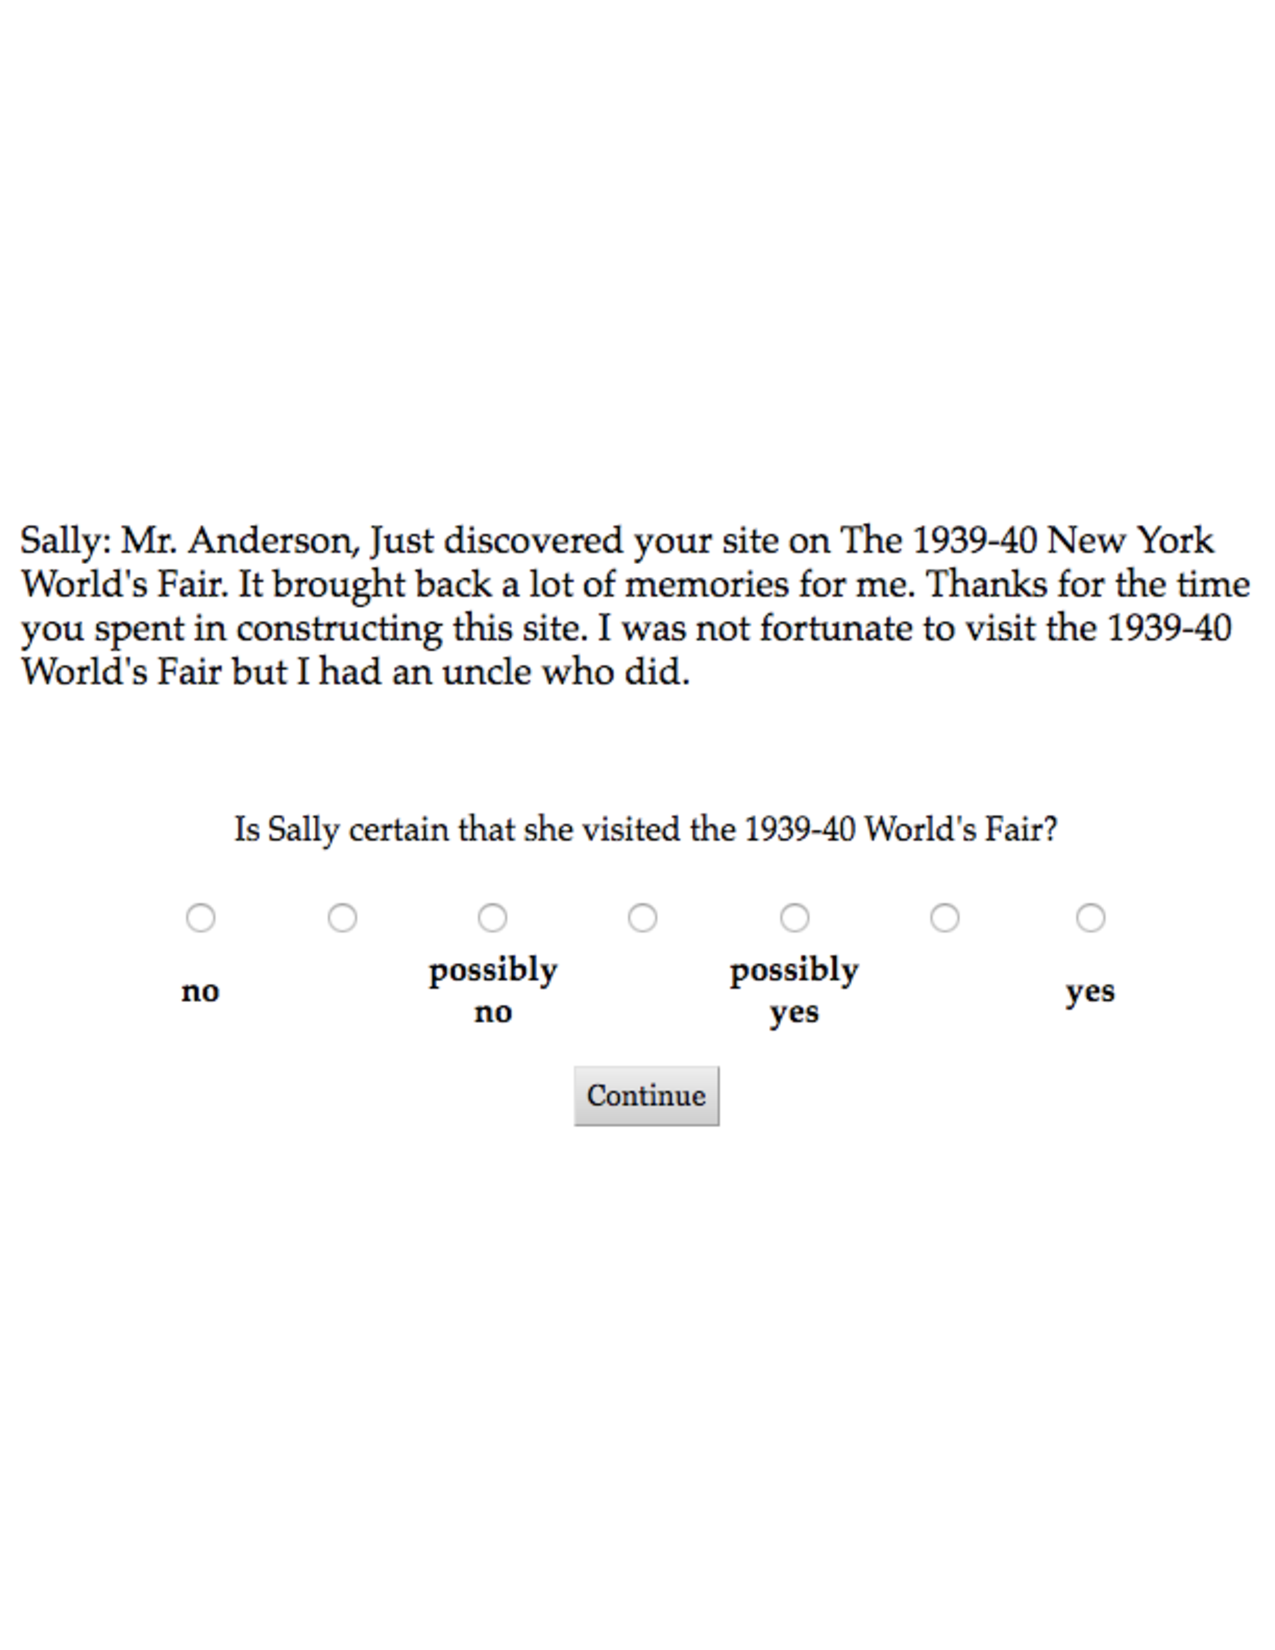
\includegraphics[width=10cm]{figures/f-corpus-trial}}
\end{center}
\caption{A sample trial in Experiment 1}\label{f-corpus-trial}
\end{figure}

After responding to the 10 stimuli, 
participants filled out a brief questionnaire about their age, their
native language(s) and, if English is a native language, whether it is
American English, as opposed to e.g., Indian or Australian English.
Participants were told that they would be paid no matter how they
responded to these questions, in order to encourage them to answer
truthfully. 

\paragraph{Data exclusion} The responses from 6 participants who did not self-identify as native speakers of American English were excluded. 28 participants gave a rating higher than 3 to the control stimulus in (\ref{cntrl}a), for which we hypothesized that participants would not take the speaker to be committed to the relevant content, or a rating lower than 5 to the control stimulus in (\ref{cntrl}b), for which we hypothesized that participants would take the speaker to be committed to the relevant content. These responses suggest that these participants were not attending to the task or interpreted the task differently. We therefore also excluded the data from these 28 participants, leaving data from 226 participants (ages: 18-83; mean: 35).

\subsection{Results and discussion}

There were 26-32 certainty ratings for each of the 59 NEAS (mean: 28.5), except for the five NEASs that appeared on two lists, for which there were 52-58 certainty ratings each (mean: 54). We calculated the mean certainty rating of the prejacent of each NEAS: the lowest mean certainty rating was 1.2, the highest was 6.7 and the mean certainty rating overall was 3.2. Given that participants gave their ratings on a 7-point scale, with the lowest rating (1) indicating that the speaker was taken to not be certain about the relevant content and the highest rating (7) indicating that the speaker was taken to be certain about the relevant content, this mean certainty rating of 3.2 already suggests that the prejacent of naturally occurring NEAS is not highly projective. Figure \ref{f-corpus} shows the mean certainty rating of each NEAS by evaluative adjective. The distribution of mean certainty ratings again suggests that the prejacent of naturally occurring NEASs is projective, but not highly so, and that NEASs in which the prejacent does not project are well-attested in naturally occurring data. These findings provide empirical support for an analysis according to which the prejacent is not lexically specified as a presupposition. 

\begin{figure}[h!]
\centering

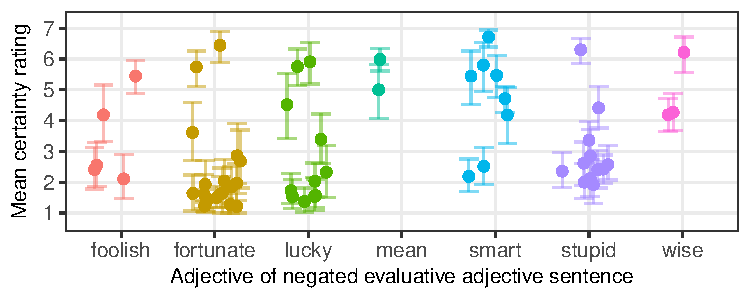
\includegraphics[width=.7\paperwidth]{../exp1-corpus-study/graphs/mean-response-by-item-and-adj}

\caption{Mean certainty ratings of 59 naturally occurring NEASs by evaluative adjective. Dotted error bars indicate bootstrapped 95\% confidence intervals.}\label{f-corpus}

\end{figure}

In (\ref{stupid}) to (\ref{smart}), we provide naturally occurring NEASs with a highly projective prejacent (a.-examples) and with a prejacent whose projectivity is very low (b.-examples); the bold-faced number included
with each example is the mean certainty rating of the prejacent.\footnote{\citet{karttunen2013}
assumed that NEAS with the  adjectives {\em
lucky, fortunate, unlucky} and {\em unfortunate} in the non-future
tenses only give rise to non-projecting interpretations; projecting
interpretations were attributed to meta-linguistic negation. Since
examples like (\ref{fort}a) cannot reasonably be attributed to
meta-linguistic negation, we continue to treat these adjectives as being compatible with 
both projecting and non-projecting interpretations (see also \citealt{karttunen-etal2014}).} Importantly, the a.- and b.-examples in (\ref{stupid}) to (\ref{smart}) differ not only in whether the prejacent projects over negation, but also in the evaluation: in the a.-examples, the evaluation is negated and in the b.-examples it is counterfactual. In (\ref{stupid}a), for instance, the evaluation is that it is not the case that God is stupid to think that his solutions work. In (\ref{stupid}b), on the other hand, the evaluation is that the Google founders would have been stupid to take on that liability.
 


%Problematic result
%\ex Zidan was once again the goalscorer for Mainz as he scored their only goal in the 81st minute. The Egyptian also had two chances in the first half but wasn't lucky to score. [4.5]

\begin{exe}


\ex\label{stupid} {\em stupid}

\begin{xlist}

\ex God offers Hope to Hispanics! In His pages are solutions to every immigration problem. God loves citizens and immigrants equally. His solutions are for all of us. They are practical. They work. He is not stupid to think so. \hfill {\bf [6.3]}

\ex There is no chance a true large scale museum can be built. The federal government cannot take on the humongous legal liability for such a hazardous site. The Google founders are not stupid to take on that liability either. \hfill {\bf [1.9]}

\end{xlist}

\ex\label{fort} {\em fortunate}

\begin{xlist}

\ex Four months after her last Prolotherapy treatment  Tessie is still
doing great. But what would have happened if she was not
fortunate to be married to Joe? \hfill {\bf [6.4]}

\ex\label{fair}  Mr. Anderson  Just discovered your site on The 1939-40 New York World's Fair. It brought back a lot of memories for me. Thanks for the time you spent in constructing this site. I was not fortunate to visit the 1939-40 World's Fair but I had an uncle who did \hfill {\bf [1.2]}

\end{xlist}

\ex\label{lucky} {\em lucky}

\begin{xlist}

\ex Not even a 40 foot ladder could reach this roof  so I had to use a boom (bucket) lift. I got a 60' lift for this particular job  and it worked out nicely. I took the above photo while working in the lift. You can see the tiles. They look nice and neat in the photo  but up close  they were riddled with gaps. I spent a great deal of time sealing them. I was lucky to have level and relatively unobstructed ground. I was not lucky to have recent rains and a several ton machine to drive on the soft ground. \hfill {\bf [5.9]}

%\ex  It seems that there is not a specific test kit to certificate thin client  or  if existing  i was not \fbox{lucky} to find it. \hfill {\bf [1.5]}

\ex Alice: Good day. My husband and i were married for four years now but before that he already has a child with his ex gf. We are not lucky to have a child of our own. \hfill {\bf [1.4]}

\end{xlist}


\ex {\em foolish}

\begin{xlist} \ex Out east in St. Bernard Parish Chad Blanchard is
hoping he was not foolish to spend his savings on reopening
Charlie's restaurant -- leaving himself with just 15 dollar bills in his
back pocket. \\ \hspace*{.1cm} \hfill {\bf [5.4]}

%\ex Archbishop Williams categorically pointed out that none of the people he had trained to become pastors could rub shoulders with him for the reason that he did not impart all of his knowledge on them. He emphasized that he was not \fbox{foolish} to give all that he had as a celebrated man of God to the people he trained  because he knew for a fact that when he did that the people could one day rub shoulders with him. \hfill {\bf [2.6]}

\ex Olmert is a dinosaur politician  he will exist for a long time in politics  and therefore will not be foolish to make the same mistake twice. \hfill {\bf [2.1]}

\end{xlist}

\ex\label{smart} {\em smart}

\begin{xlist}

\ex I think Mark Cuban was not smart to let a successful coach go in Avery Johnson. \hfill {\bf [6.7]}

%\ex You and I must trust God for our finances  but that's no license to
%spend sillily. You and I ought to trust God for safety in the car  but
%we are not \fbox{smart} to pass on a blind curve. \hfill {\bf [2.5]}

\ex Once you installed this free Notipage webpage monitoring software
then just make your first alert. It's worth mentioning here that the app
will not be smart to keep an eye on web pages that are only easy
to get to by logging in to a site or service.   \hfill {\bf [2.2]}

\end{xlist}

\end{exe}

In sum, our study of naturally occurring NEASs shows that the prejacent is not highly projective. These findings converge with those of \citet{tbd-variability}, who studied the projectivity of a variety of utterance contents and found that the prejacent of four (constructed) polar interrogative EASs with {\em stupid} was significantly less projective than the content of the clausal complement of the emotive predicate {\em be annoyed} and the cognitive predicate {\em know}. In the next section, we develop an analysis according to which the projectivity of the prejacent is not due to its lexical status as a presupposition but instead derived from the question that the utterance of the EAS is taken to address. 
 

\section{A question-based analysis of the projectivity of the prejacent}\label{s3}

In this section, we develop an analysis according to which the projectivity of the prejacent of an utterance of an EAS is derived from its status relative to the question addressed by the utterance. Specifically, we propose that the prejacent projects when it is not at-issue with respect to the question addressed by the utterance (see, e.g., \citealt{brst-salt10,brst-ar,best-question}). To understand which questions EASs can address, we first consider the lexical entailments of EASs.

\subsection{Lexical entailments of evaluative adjective sentences}\label{s31}

We propose that an unembedded EAS has (at least) two lexical entailments: the prejacent and what we refer to as the `generalization'. As shown in (\ref{ent}), the generalization is timeless and the tense of the EAS ({\sc tense}) determines the temporal reference of the prejacent.

\begin{exe}
\ex\label{ent} Two lexical entailments of unembedded evaluative adjective sentences `NP be{\sc .tense} Adj to VP'\footnote{Some EASs with {\em will} appear to not entail the prejacent: for example, some speakers do not judge (i) to entail that Johnson will take what he can get. We thank David Beaver (p.c.) for this point, which we sidestep here.
\begin{exe}
\exi{(i)} With more teams denying interest in Johnson, he will be smart
to take what he can get. \\ ({\em http://www.sportsworldreport.com/articles/28999/20140407/chris-johnson-rumors-ny-jets-release-mike-goodson-free-agent-signs-dallas-cowboys-demarco-murray-rams-falcons.htm})
\end{exe}} 

\begin{xlist}

\ex Generalization: In VPing NP is/would be Adj

\ex Prejacent: NP VP{\sc .tense}

\end{xlist}
\end{exe}
By (\ref{ent}), a past tense EAS like (\ref{f}) {\em Feynman was stupid to dance on the table} entails that, in dancing on the table, Feynman is/would be stupid (the generalization) and that Feynman danced on the table (the prejacent). Likewise, a present tense EAS like the non-negated variant of (\ref{stupid}b) {\em God is stupid to think that his solutions work} entails that, in thinking that his solutions work, God is/would be stupid (the generalization) and that God thinks that his solutions work (the prejacent). The generalization is timeless and attributes the property denoted by the evaluative adjective Adj to the referent of the subject NP relative to events of the type denoted by the VP. These events may, but need not be, actual: for instance, it does not follow from the generalization of (\ref{f}) that an event of Feynman dancing on the table took place.

In contrast to the generalization and the prejacent, we do not take the evaluation to be a lexical entailment of EASs (unlike, e.g., \citealt{barker02}). However, for unembedded EASs, the evaluation follows straightforwardly from the lexical entailments. For instance, in (\ref{f}), the evaluation that Feynman was stupid to dance on the table follows from the generalization, that in dancing on the table Feynman is/would be stupid, and the prejacent, that Feynman danced on the table. To preview the proposal: when an EAS is embedded under an entailment-canceling operator, it is not the case that both of the lexical entailments survive as commitments of the speaker. As a consequence, what follows from such EASs differs, thus capturing, as we show below, that the evaluation of such EASs depends on which content projects, i.e., is a commitment of the speaker.

The proposal in (\ref{ent}), according to which the prejacent and the generalization are lexical entailments, predicts that unembedded EASs are judged to be unacceptable if either entailment is false. The examples in (\ref{false}) show that that prediction is borne out. Consider (\ref{false}a), whose prejacent is false and whose generalization is true (under the assumption that anybody, including Kim, being born into poverty is unfortunate): this example is correctly predicted to be unacceptable because the prejacent is false. In (\ref{false}b), on the other hand, the prejacent is true and the generalization is false (under the assumption that it is not the case that anybody, including Sandy, being born into poverty is lucky). This sentence is correctly predicted to be judged to be unacceptable because the generalization is false. 

\begin{exe}
\ex\label{false}
\begin{xlist}
\ex What is true: Kim was born to rich parents
\\ \infelic Kim was unfortunate to be born into poverty.

\ex What is true: Sandy was born into poverty
\\ \infelic Sandy was lucky to be born into poverty.

\end{xlist}
\end{exe}

The generalization of an EAS involves the meaning of the (positive) evaluative adjective, whose meaning depends on a contextual standard (e.g., \citealt{kennedy2001}). Our examples in (\ref{false}) appealed to a contextual standard for {\em unfortunate} and {\em lucky} such that any reader would agree that somebody being born into poverty counts as unfortunate and doesn't count as lucky; more elaborately: the degree to which somebody being born into poverty is unfortunate is higher than the contextual standard for {\em unfortunate} and the degree to which somebody being born into poverty is lucky is lower than the contextual standard for {\em lucky}. What follows from the common ground, which we assume includes world knowledge, is that the generalization of (\ref{false}a), that in being born into poverty Kim is/would be unfortunate, is true and the generalization of (\ref{false}b), that in being born into poverty Sandy is/would be lucky, is false. 

The common ground does not always determine whether the generalization of an EAS is true or false. Consider, for instance, the generalization that, in buying the Xbox 360 Elite, a particular individual $x$ is/would be stupid. Whether this generalization is true or false depends on $x$'s personal circumstances, such as how much money they have, whether they are addicted to gaming and shouldn't be tempted any further, or whether the Xbox is a present for somebody else. Common ground information does not suffice to identify whether the generalization is true or false; we refer to such generalizations as `neutral'. As a consequence, when a speaker utters the EAS in (\ref{xbox}), the generalization, that in buying the Xbox 360 Elite the speaker is/would be stupid, is new information that the speaker is committing to as true: the speaker informs the addressee that the degree to which them buying an Xbox 360 Elite is stupid is higher than the contextual standard of {\em stupid} (see also \citealt{barker02} for this point). For other speakers, this generalization may be false, in which case they could not truthfully utter (\ref{xbox}).

\begin{exe}
\ex\label{xbox} I was stupid to buy the Xbox 360 elite.\footnote{\url{www.gamespot.com/forums/xbox-association-1000003/i-was-stupid-to-buy-the-xbox-360-elite-26937557}}
\end{exe}

The examples in (\ref{false}) and (\ref{xbox}) illustrate that the generalizations of EASs come in different flavors. At one extreme are generalizations whose truth follows from the common ground, like `in being born into poverty Kim is/would be unfortunate' in (\ref{false}a). At the other extreme are generalizations whose falsity follows from the common ground, like `in being born into poverty Sandy is/would be lucky' in (\ref{false}b). In addition to generalizations at these two extremes, there are also, of course, generalizations at any point in-between: given the common ground, some generalizations are more likely to be true than others. Neutral generalizations, whose truth or falsity does not follow from the common ground, are an example of generalizations between these two extremes. In this paper, we argue that the strength of the inference from the common ground to the truth of the generalization is a key factor in identifying the interpretation of EASs, including the projectivity of the prejacent. In the next section, we discuss the role that the question that an utterance of an EAS addresses plays in the interpretation of the utterance.

\subsection{At-issue content of utterances of evaluative adjective sentences}\label{s32}

Although an utterance typically conveys several contents, only one of these contents is the main point of the utterance, i.e., what the utterance is about (\citealt{potts05}). We refer to the content that an utterance is about as the `at-issue' content and characterize at-issue content on the basis of the `Discourse Question' (\citealt{best-question}), i.e., the (explicit or implicit) question that provides the topic of a segment of discourse. At-issue content is content that addresses the Discourse Question (see, e.g., \citealt{brst-salt10,brst-ar}).

Consider, for instance, the content of the clausal complement of {\em discover} in B's utterance in (\ref{discover2}a) and (\ref{discover2}b), that Harriet was at Princeton for a job interview. In these examples, the Discourse Questions that B's utterances address are made explicit by A's interrogative utterances. In (\ref{discover2}a), the content of the clausal complement of {\em discover} is at-issue because it addresses the Discourse Question: that Harriet was at Princeton for a job interview is an answer A's interrogative utterance of where Harriet was yesterday. In (\ref{discover2}b), on the other hand, the content of the clausal complement of {\em discover} is not-at-issue because it is not an answer to A's interrogative utterance; rather, here the Discourse Question is addressed by the main clause content of B's utterance.


\begin{exe}
\ex\label{discover2}
\begin{xlist}
\ex
\begin{xlist}
\exi{A:} Where was Harriet yesterday?
\exi{B:} Henry discovered that she was at Princeton for a job interview.
\end{xlist}

\ex
\begin{xlist}
\exi{A:} Why is Henry in such a bad mood?
\exi{B:} He discovered that Harriet was at Princeton for a job interview.
\\ \hspace*{.2cm} \hfill (examples adapted from \citealt[1035]{simons07})
\end{xlist}

\end{xlist}
\end{exe}

The examples in (\ref{ai}) illustrate four Discourse Questions that utterances of EASs can address. These Discourse Questions show that both lexical entailments of EASs, the prejacent and the generalization, can be at-issue. The Discourse Questions in (\ref{ai}a) and (\ref{ai}b) are about the prejacent: both the question of whether Sam got a ticket in (\ref{ai}a) and who got a ticket in (\ref{ai}b) are answered by the prejacent of B's utterances, that Sam got a ticket.\footnote{Some native speakers of American English may not judge B's utterances in (\ref{ai}a) and (\ref{ai}b) to be acceptable and prefer versions with {\em enough}: {\em She was smart enough to buy one the day they went on sale}. We hypothesize that such judgments of unacceptability are due to such speakers dispreferring EAS in which the prejacent is at-issue. Given the hypothesis we advance below, that the prejacent projects to the extent that it is not at-issue, we expect such speakers to also judge NEAS like (\ref{nat}) in which the prejacent does not project to be unacceptable. Crucially, however, even speakers who prefer to realize (\ref{ai}a) and (\ref{ai}b) with {\em enough} can retrieve the intended interpretations of the variants without {\em enough}.} Thus, in (\ref{ai}a) and (\ref{ai}b), the prejacent is at-issue and the generalization, that in buying a ticket the day the tickets went on sale Sam is be smart, is not at-issue. The Discourse Questions in (\ref{ai}c) and (\ref{ai}d), on the other hand, are not about the prejacent:  both the question of how Sam got a ticket in (\ref{ai}c) and whether Sam was smart to buy a ticket the day they went on sale in (\ref{ai}d) are not answered by the prejacent of B's utterances, that Sam got a ticket, but by the generalization, that in buying a ticket the day the tickets went on sale Sam is smart. Thus, in (\ref{ai}c) and (\ref{ai}d), the generalization is at-issue and the prejacent is not at-issue.

\begin{exe}
\ex\label{ai}

\begin{xlist}
\ex
\begin{xlist}
\exi{A:} The show was sold out. Did Sam get a ticket?
\exi{B:} She was smart to buy one the day they went on sale.
\end{xlist}

\ex
\begin{xlist}
\exi{A:} There were so few tickets for the show! Who got a ticket?

\exi{B:} Sam was smart to buy one the day they went on sale. 

\end{xlist}

\ex
\begin{xlist}
\exi{A:} The tickets for the show sold out really quickly! How did Sam get a ticket?

\exi{B:} Sam was smart to buy one the day they went on sale.

\end{xlist}

\ex
\begin{xlist}
\exi{A:} Was Sam smart to buy a ticket for the show the day the tickets went on sale? The price would have gone down after a few days!

\exi{B:} Sam was smart to buy one the day they went on sale. The show sold out the day the tickets went on sale.

\end{xlist}

\end{xlist}
\end{exe}

Identifying which utterance content is at-issue is critical not only to understanding what the utterance is about, but also because of the connection between at-issueness and projectivity (e.g., \citealt{potts05,brst-salt10,best-question,brst-ar}). For EAS, identifying whether the prejacent or the generalization are at-issue thus also plays a role in identifying whether the prejacent projects, as we discuss next.

\subsection{The prejacent projects when it is not at-issue with respect to the Discourse Question}

As mentioned above, we do not assume that the prejacent is lexically specified as a presupposition. Rather, we propose that the projectivity of the prejacent of an utterance of an EAS is derived from the discourse status of the prejacent. Specifically, we argue that the prejacent projects if and only if it is not at-issue with respect to the Discourse Question addressed by the utterance. 

To illustrate the proposal, consider the examples in (\ref{ai2}a) and (\ref{ai2}b), where B utters NEASs. The prejacent is at-issue in (\ref{ai2}a) because A's interrogative utterance, assumed to be the Discourse Question, is about the prejacent. Thus, according to our proposal, the prejacent of B's utterance in (\ref{ai2}a) is predicted to not project: accordingly, B's utterance means that Sam didn't buy a ticket the day they went on sale (the prejacent does not project) and that buying a ticket the day they went on sale would have been smart for Sam. In (\ref{ai2}b), on the other hand, A's interrogative utterance, is about the generalization. Thus, the prejacent of B's utterance is not at-issue and, according to our proposal, is predicted to project. Accordingly, B's utterance is interpreted to mean that Sam bought a ticket the day they went on sale and that Sam buying a ticket the day they went on sale wasn't smart. 


\begin{exe}
\ex\label{ai2}

\begin{xlist}
\ex
\begin{xlist}
\exi{A:} The show was sold out. Did Sam get a ticket?
\exi{B:} She wasn't smart to buy one the day they went on sale. (So, she didn't go to the show.)
\end{xlist}

\ex
\begin{xlist}
\exi{A:} Was Sam smart to buy a ticket for the show the day the tickets went on sale? The price would have gone down after a few days!

\exi{B:} Sam wasn't smart to buy one the day they went on sale. The price indeed went down after a few days.

\end{xlist}

\end{xlist}
\end{exe}

As mentioned above, we take projectivity to be a gradient property of utterance content rather than a binary, categorical one. This assumption is motivated by experimental findings reported on in \citealt{tbd-variability} as well as the corpus study reported on in section \ref{s2}, which showed that authors can be taken to be committed to the prejacent of NEASs to varying degrees. Thus, we assume that what it means for projectivity to be a gradient property is that a reader's (or listener's) judgment that a content is projective to a certain extent means that the reader takes the author (or speaker) to be committed to the content to that extent. On this interpretation, projectivity being a gradient property is a consequence of author (or speaker) commitment being a gradient property (for discussion, see \citealt{tbd-variability}). Accordingly, to capture the relation between projectivity and not-at-issueness, we assume \citepos{tbd-variability} Gradient Projection Principle:\footnote{The question of why not-at-issue content projects has received several different answers. \citet{brst-salt10} proposed that not-at-issue content is not targeted by operators, such as negation, thereby resulting in the content projecting over such operators. In this paper, we follow \citet{abrusan2011} in assuming that the not-at-issue content is backgrounded and projects as a result of its discourse status.}

\begin{exe}
\ex\label{gpp} {\bf Gradient Projection Principle:} If content $C$ is expressed by a constituent embedded under an entailment-canceling operator, then $C$ projects to the 
extent that it is not at-issue.

\end{exe}

Preliminary evidence that the projectivity of the prejacent of EASs depends on its at-issueness comes from \citealt{tbd-variability}, who investigated the Gradient Projection Principle on the basis of 19 projective contents associated with American English expressions. \citet{tbd-variability} collected both projectivity and at-issueness ratings for these 19 contents, one of which was the prejacent of EASs with {\em stupid} embedded under the polar question operator. The four evaluative adjective polar questions studied in their work are given in (\ref{stupid2}):

\begin{exe}
\ex\label{stupid2}

\begin{xlist}

\ex Was Raul stupid to cheat on his wife?

\ex Were John's kids stupid to be in the garage?

\ex Is Mary's daughter stupid to be biting her nails?

\ex Is Richie stupid to be a stuntman? \hfill (\citealt{tbd-variability}, Appendix A)

\end{xlist}

\end{exe}


Figure \ref{f-corr} shows participants' projectivity ratings for the prejacents of the four polar questions in (\ref{stupid2}) against their not-at-issueness ratings. There is a clear relationship between at-issueness and projectivity: the more a participant rated a prejacent as not-at-issue, the more projective they rated it ($r =$ .91; when not collapsing over the four polar questions $r =$ .57). This finding provides preliminary evidence that the projectivity of the prejacent is sensitive to its at-issueness.

\begin{figure}[h!]
\centering

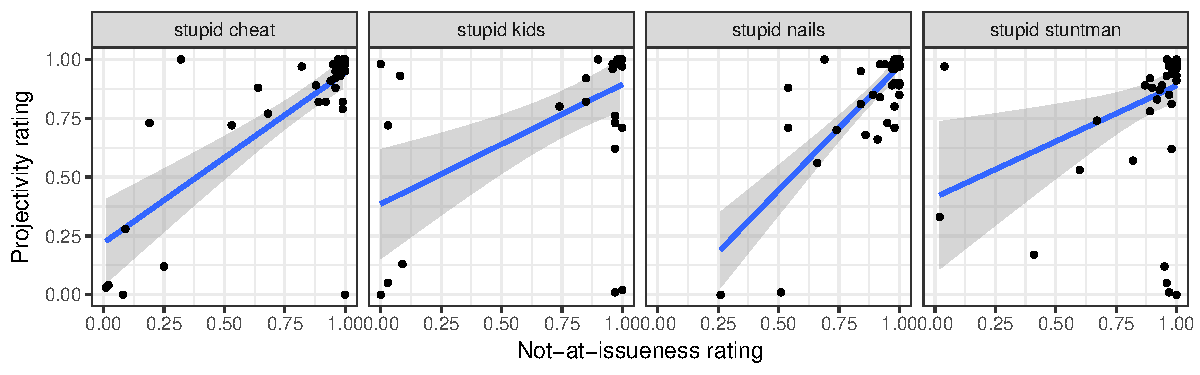
\includegraphics[width=1\textwidth]{figures/Exp1a-subject-projai-stupid}

\caption{Projectivity ratings against not-at-issueness ratings for the prejacent of the four polar question EASs in \citealt{tbd-variability}. Each dot represents one participant's ratings. Linear smoothers with 95\% confidence intervals overlaid.}
\label{f-corr}
\end{figure}

In \citepos{tbd-variability} experiment, the evaluative adjective polar questions in (\ref{stupid2}) were not presented as responses to interrogative utterances that made the Discourse Questions explicit. Rather, participants were asked to imagine that the polar questions were uttered by speakers who they overhear at a party. The absence of an explicit Discourse Question is, of course, not unusual and rather the norm in naturally occurring data. Given the importance of the Discourse Question to the interpretation of EASs, in particular the at-issueness of the prejacent, we need to understand how the Discourse Question of utterances not presented in response to an interrogative utterance is constrained. In this paper, we consider two cues to the Discourse Questions of utterances of EASs: the information structure of the utterance (section \ref{s331}) and the discourse status of the generalization (section \ref{s332}).\footnote{\citet{abrusan2011} proposed that entailments of utterances that are about the running time of the main event are the default main point, i.e., what we have referred to as the at-issue content. However, given Abrus\'an's notion of aboutness, both the prejacent and the generalization of EASs are about the running time of the main event. For instance, \citet[508]{abrusan2011} took the entailment of (i), that John solved the exercise, to be ``non-accidentally (i.e. necessarily) about the matrix event time''. By the same argument, the prejacent of (ii) would be about the matrix event time, which means that neither the prejacent nor the generalization are predicted by \citealt{abrusan2011} to be the default at-issue content of EASs.



\begin{exe}
\exi{(i)} John managed (at time t$_{\mbox{1}}$) to solve the exercise (at t$_{\mbox{1}}$). \hfill (\citealt[508]{abrusan2011})

\exi{(ii)} John was smart (at time t$_{\mbox{1}}$) to solve the exercise (at t$_{\mbox{1}}$).

\end{exe}}


\subsubsection{Information-structural focus}\label{s331}

In this section, we argue that the information structure of an utterance of an EAS provides a cue to the Discourse Question addressed and, thereby, to the at-issueness of the prejacent. 

The relationship between information structure and Discourse Questions is indirect, via  the so-called Current Question (see \citealt{beaver-clark08,best-question,brst-ar}). The Current Question is derived from the focus marking of the utterance (as illustrated below) and constrains the Discourse Question in that the two questions must form a strategy of inquiry (Roberts 1998/2012\nocite{roberts98,roberts12}). Thus, what we propose, following \citealt{best-question}, is that i) the prosodic realization of the utterance of an EAS provides a cue to what is focused, ii) what is focused, in turn, constrains the Current Question of the utterance, and iii) the Current Question constrains the Discourse Question. We proceed bottom-up in identifying how the information structure of the utterance constrains the Discourse Question. 

Our starting point is the long-standing observation that utterances must be congruent with the interrogative utterances
they address (e.g., \citealt{paul1880,paul1919,vstechow90,rooth92}). The
question-answer pairs in (\ref{qa}) illustrate
question-answer congruence: J's utterance in (\ref{qa1}), with {\em
Turkish} prosodically prominent (as indicated by capital letters), is congruent with M's question in
(\ref{qa1}), but not with M's question in (\ref{qa2}), and vice versa
for J's utterance in (\ref{qa2}), where {\em David} is prosodically
prominent.

\begin{exe} 

\ex\label{qa} David, Mandy, Craige and Judith are eating at a place that serves Turkish, Lebanese and Irish coffee.

\begin{xlist} 

\ex\label{qa1} 

\begin{xlist}

\exi{M:} What kind of coffee does David like? 

\exi{J:} David likes TURkish coffee.

\end{xlist}

\ex\label{qa2}

\begin{xlist}

\exi{M:} Who likes Turkish coffee?

\exi{J:} DAvid likes Turkish coffee. \hfill (adapted from \citealt[951]{tonhauser-salt26})

\end{xlist}

\end{xlist}
\end{exe}

Question-answer congruence is straightforwardly modeled in an
alternative semantics framework (see, e.g., \citealt{rooth85,rooth92}), which
analyzes both the focus semantic meaning of the answer and the meaning of
the question in terms of alternatives. In such a framework, the meanings
of the questions in (\ref{qa1}) and (\ref{qa2}) are sets of propositions
that are answers to the questions, as shown in (\ref{cong1}a) and
(\ref{cong2}a), respectively. The focus
semantic meanings of the answers in (\ref{qa1}J) and (\ref{qa2}J) are
focus alternatives sets, i.e., sets of propositions derived by
abstracting over the focused expressions, as shown in (\ref{cong1}b) and
(\ref{cong2}b).

\begin{exe}
\ex\label{cong1}

\begin{xlist}

\ex \sem{(\ref{qa1}M)}{M,g} = \{David likes Turkish coffee, David likes Lebanese coffee, David likes Irish coffee\}

\ex \sem{(\ref{qa1}J)}{M,g} = \{David likes Turkish coffee, David likes Lebanese coffee, David likes Irish coffee, David likes cold coffee,\ldots\} 

\end{xlist}

\ex\label{cong2}

\begin{xlist}

\ex \sem{(\ref{qa2}M)}{M,g} = \{David likes Turkish coffee, Craige likes Turkish coffee, Mandy likes Turkish coffee, Judith likes Turkish coffee\}

\ex \sem{(\ref{qa2}J)}{M,g} = \{David likes Turkish coffee, Craige likes Turkish coffee, Mandy likes Turkish coffee, Judith likes Turkish coffee, Adam likes Turkish coffee,\ldots\}

\end{xlist}

\end{exe} The observation that answers are congruent with the questions
they address is modeled by requiring the meaning of the question to be a
subset of the focus alternatives set of the answer. For instance, the
answer in (\ref{qa1}J) is congruent with the question in (\ref{qa1}M)
because the meaning of the question, given in (\ref{cong1}a), is a
subset of the meaning of the answer, given in (\ref{cong1}b). The
answer in (\ref{qa1}J) is not congruent with the question in
(\ref{qa1}M) because the meaning of the question, given in
(\ref{cong2}a), is not a subset of the meaning of the answer. 

From the requirement of question-answer congruence it follows that the prosodic realization of an utterance not made in response to an interrogative utterance provides a cue to the question addressed by the utterance. Experimental evidence comes from, for instance, \citealt{most-saltz79}, who found that listeners rely on the location of pitch accents in utterances of sentences like {\em The pitcher threw the ball} in identifying whether the subject or the object is focused. In one of their experiments, participants listened to utterances of such sentences in which either the subject or the object was prosodically prominent and were asked to write a question to which the utterance would be an appropriate answer. Most and Saltz found that the expression that was prominent in the answer utterance corresponded, in 68\% of cases, to the expression that was focused in the utterance, given the question that the participant had provided. For instance, the question {\em Who threw the ball?} was written for the utterance {\em The pitcher threw the ball} in which the subject was prosodically prominent. For further relevant evidence and comments see, e.g., \citealt{halliday67,birch-clifton1995} and \citealt{breen-etal10}. 

The Current Question of an utterance is defined as a subset of the focus alternative set of the utterance, thereby ensuring that the utterance is congruent to its Current Question:

\begin{exe} \ex\label{cq}  The
{\bf Current Question} of an utterance is a privileged subset of the focus
alternatives set of the uttered sentence (given a structural analysis of
that sentence, including focus marking) which meets the following
conditions:

\begin{xlist}
\exi{(i)} The proposition expressed is a member of the Current Question and
\exi{(ii)} The Current Question has at least one additional member. \hfill (\citealt[194]{best-question})
\end{xlist}

\end{exe}

To illustrate this definition, consider J's utterance in (\ref{qa}a). The focus alternative set of this utterance, given its focus marking, is a set of propositions that varies over the focused expression, namely (\ref{cong1}b). Per (\ref{cq}), the Current Question of the utterance is a subset of this focus alternative set. Given that the context of (\ref{qa}a) is restricted to Turkish, Lebanese and Irish coffee, the Current Question of (\ref{qa}a) is that subset of (\ref{cong1}b) that is restricted to these types of coffees, i.e., the meaning of the interrogative utterance in (\ref{cong1}a). Likewise, the Current Question of J's utterance in (\ref{qa}b) is a subset of the focus alternative set given in (\ref{cong2}b), namely the meaning of the interrogative utterance in (\ref{cong2}a). Both Current Questions include the proposition expressed by the utterance (that David likes Turkish coffee) but they differ on their additional members.

Having shown how the prosodic realization of an utterance provides a cue to its  Current Question, we now return to EASs. A complete analysis of the Current Questions of such sentences would require of a full specification of how the prosody of utterances of EASs constrains what is focused in the utterances. Such an analysis cannot be given at this point because  the connection between prosody and focus with EASs is much less well-understood than with the simple subject-verb-object sentences considered above. We therefore limit ourselves to four cases that illustrate the cue that prosody provides to the Current Questions of utterances of EASs. The four cases are given in (\ref{vp}) to (\ref{aux}). In the a.-examples, we indicate which expression is focused using the [\hspace*{.1cm}]\foc{} notation and also provide a prosodic realization of the utterance (in the form of  ToBI annotations)\footnote{In the Tone and Break Indices annotation system (ToBI,
\citealt{beckman-ayers97}), H* is a
high tone pitch accent aligned with the stressed syllable and L+H*  is a
complex pitch accent made up of a high tone aligned with the stressed
syllable and an immediately preceding low tone. A low intermediate phrase accent
that is followed by a low intonational phrase boundary tone is indicated
by L-L\% .} that is compatible with the indicated focus marking. In the b.-examples, we give the corresponding focus alternative sets. For instance, in (\ref{np}), where the subject is focused, the focus alternative set of the utterance is a set of propositions of the form `$x$ was smart to buy a ticket the day they went on sale', with $x$ some entity.


\begin{exe}

\ex\label{vp}

\begin{xlist}

\ex Sam was smart [to buy a ticket the day they went on SALE]\foc.
\\
\hspace*{1.8cm} H* \hspace*{5.8cm} H* \hspace*{.4cm} L-L\%

\ex \{Sam was smart to buy a ticket the day they went on sale, Sam was smart to bring her wallet, Sam was smart to learn French,\ldots\}


\end{xlist}

\ex\label{np} 
\begin{xlist}

\ex {[}SAM]\foc{} was smart to buy a ticket the day they went on sale.  \\
L+H* \hspace*{8cm} L-L\%

\ex \{Sam was smart to buy a ticket the day they went on sale, Mary was smart to buy a ticket the day they went on sale, Sue was smart to buy a ticket the day they went on sale,\ldots\}

\end{xlist}


\ex\label{adj}

\begin{xlist}

\ex Sam was [SMART]\foc{} to buy a ticket the day they went on sale.
\\
\hspace*{1.6cm} L+H* \hspace*{6.5cm} L-L\%

\ex \{Sam was smart to buy a ticket the day they went on sale, Sam was clever to buy a ticket the day they went on sale, Sam was wise to buy a ticket the day they went on sale,\ldots\}


\end{xlist}

\ex\label{aux} 

\begin{xlist}

\ex Sam [WAS]\foc{} smart to buy a ticket the day they went on sale.
\\
\hspace*{.8cm} L+H* \hspace*{7.2cm} L-L\%

\ex \{Sam was smart to buy a ticket the day they went on sale, it is not the case that Sam was smart to buy a ticket the day they went on sale\}
 
\end{xlist}


\end{exe}
From the definition in (\ref{cq}) it follows that the Current Questions of the utterances of the EASs in (\ref{vp}a) to (\ref{aux}a) are subsets of the focus alternative sets in (\ref{vp}b) to (\ref{aux}b), respectively. That is, utterances of the EASs in (\ref{vp}a) to (\ref{aux}a) are taken to address Current Questions that are subsets of the focus alternative sets in (\ref{vp}b) to (\ref{aux}b), respectively.

What is important to realize is that these Current Questions differ in their entailments (where a question entails a proposition if every alternative of the question entails that proposition). Entailments of the Current Questions (CQs) of the utterances in (\ref{vp}a) to (\ref{aux}a) are given in (\ref{entail}):

\begin{exe}
\ex\label{entail}

\begin{xlist}

\ex CQ of (\ref{vp}a), a subset of (\ref{vp}b), entails that, in doing something, Sam was smart.

\ex CQ of (\ref{np}a), a subset of (\ref{np}b), entails that somebody bought a ticket the day they went on sale and that, in buying a ticket the day they went on sale, somebody was smart.

\ex CQ of (\ref{adj}a), a subset of (\ref{adj}b), entails that in buying a ticket the day they went on sale Sam had some property.

\ex CQ of (\ref{aux}a), a subset of (\ref{aux}b), entails that Sam exists.

\end{xlist}

\end{exe}
What it means for these propositions to be entailed by the Current Questions of the utterances in (\ref{vp}a) to (\ref{aux}a) is that at the time at which the utterances are made, the speaker considers these entailments to already be part of the common ground of the interlocutors. For instance, when (\ref{np}a) is uttered, the proposition that somebody bought a ticket the day they went on sale and that, in buying a ticket the day they went on sale, somebody was smart is already part of the common ground or, at least, assumed to be true by the speaker. In this context, what remains to be addressed, according to the speaker, is the identity of individuals that bought a ticket and who, in buying a ticket the day they went on sale, were smart.

We are now ready to consider how the Current Question constrains the Discourse Question, which in turn determines the at-issueness of the prejacent.  Following Roberts 1998/2012\nocite{roberts98,roberts12}, we assume that the Current Question and the Discourse Question are part of a strategy of inquiry. Specifically, we assume that the Current Question is a subquestion of the Discourse Question: this means that a complete answer to the Current Question must contextually entail a partial answer to the Discourse Question. Crucially, what follows from this is that the Discourse Question must still be open, i.e., unanswered, at the time at which the utterance is made. 

To illustrate how the Current Question constrains the Discourse Question, consider an utterance of the example in (\ref{aib}), which is presented with its focus alternative set. The Current Question, as a subset of this focus alternative set, entails that somebody bought a ticket the day they went on sale and that somebody buying a ticket the day they went on sale is smart. That is, when this utterance is made, what is already taken to be part of the common ground is that somebody bought a ticket the day they went on sale and that, in buying a ticket the day they went on sale, somebody was smart. Only some Discourse Questions are plausible, given this common ground information. In particular, both the Discourse Questions `Who got a ticket?' and `Did Sam get a ticket?' are plausible because both are unanswered given the entailments of the Current Question. On the other hand, Discourse Questions like `How did Sam get a ticket?' and `Was Sam smart to buy a ticket the day they went on sale?' are less plausible because what is common ground already answers these Discourse Questions.

\begin{exe}
\ex\label{aib} {[}Sam]\foc{} was smart to buy a ticket the day they went on sale.
\\ \{Sam was smart to buy a ticket the day they went on sale, Mary was smart to buy a ticket the day they went on sale, Sue was smart to buy a ticket the day they went on sale,\ldots\}
\end{exe}
The focus marking of the utterance in (\ref{aib}) constrains the Current Question, and the entailments of the Current Question constrains the Discourse Questions. Since the plausible Discourse Questions of (\ref{aib}) are such that the prejacent of (\ref{aib}) is at-issue, this means that the information structure of (\ref{aib}) provides a cue that the prejacent is at-issue and the generalization, in turn, is not at-issue.

Next consider an utterance of the example in (\ref{aic}), again presented with its focus alternative set. The Current Question entails that Sam bought a ticket the day they went on sale and that, in buying a ticket the day they went on sale, Sam had some property. That is, when (\ref{aic}) is uttered, what is already taken to be part of the common ground is that Sam bought a ticket the day they went on sale and that, in buying a ticket the day they went on sale, Sam had some property. Both the Discourse Questions `How did Sam get a ticket?' and `Was Sam smart to buy a ticket the day they went on sale?' (according to which the prejacent is not at-issue) are plausible because the common ground information does not already answer these Discourse Questions. On the other hand, the Discourse Questions `Who got a ticket?' and `Did Sam get a ticket?' (according to which the prejacent is at-issue) are less plausible because what is taken to be common ground already answers these Discourse Questions. 

\begin{exe}
\ex\label{aic} Sam was [smart]\foc{} to buy a ticket the day they went on sale.
\\ \{Sam was smart to buy a ticket the day they went on sale, Sam was clever to buy a ticket the day they went on sale, Sam was wise to buy a ticket the day they went on sale,\ldots\}
\end{exe}
Because the plausible Discourse Questions of (\ref{aic}) are such that the prejacent of (\ref{aic}) is not at-issue, this means that the information structure of (\ref{aic}) provides a cue that the prejacent is not at-issue and the generalization, in turn, is at-issue.

In sum, this section has illustrated how the focus marking of an utterance of an EAS constrains the Discourse Question of the utterance and, thereby, the at-issueness of the prejacent. For EASs that are embedded under an entailment-canceling operator, the focus marking of utterances of such EAS is thereby predicted to influence the projectivity of the prejacent.


\subsubsection{The discourse status of the generalization}\label{s332}

A second cue to the Discourse Question of an utterance of an EAS comes, we argue, from the discourse status of the generalization, specifically the strength of the inference from the common ground to the truth of the generalization.

 Our argument builds on a felicity requirement that is found in different guises in the literature: an utterance of an indicative sentence is felicitous only if the sentence is informative in the context in which it is uttered. \citet[144]{groenendijk1999}, for instance, formulates this as the requirement that indicative sentences be non-redundant. We assume here that an utterance of an indicative sentence is informative if its at-issue content is not already entailed by the common ground of the interlocutors prior to the utterance of the sentence. No such requirement exists for not-at-issue content: some not-at-issue content, like presuppositions, may be entailed by the common ground prior to utterance and other not-at-issue content, like conventional implicatures, may even be required to not be entailed, as argued in \citealt{potts05}. 
 Crucially, what follows from the felicity requirement is that the Discourse Question of an utterance of an indicative sentence cannot be about content that is entailed by the common ground because such a Discourse Question would render the utterance uninformative. This felicity requirement is captured by the principle in (\ref{principle1}).
 
\begin{exe}
\ex\label{principle1} {\bf Non-redundancy principle for at-issue content} \\ For utterance content $c$, if $c$ is entailed by the common ground, then the Discourse Question of the utterance is not about $c$, i.e., $c$ is not the at-issue content of the utterance. 
\end{exe}

We argued in section \ref{s31} that the inference to the truth of the generalization from the common ground may be more or less strong. That is, while the truth of some generalizations may be entailed by the common ground, the strength of the inference to the truth of other generalizations may vary. To capture that inferences to utterance content from the common ground come in different strengths, we amend the principle in (\ref{principle1}) to a gradient variant:

\begin{exe}

\ex\label{principle} {\bf Gradient non-redundancy principle for at-issue content} \\ For utterance content $c$, the stronger the inference to the truth of $c$ from the common ground, the less likely is it that the Discourse Question of the utterance is about $c$, i.e., $c$ is less at-issue.

\end{exe}

For EASs, a consequence of the principle in (\ref{principle}) is that the stronger the inference to the truth of the generalization from the common ground, the less likely the Discourse Question is about the generalization, i.e., the generalization is less at-issue. Given that the prejacent is another salient lexical entailment of EASs, it follows that the less at-issue the generalization is, the more at-issue the prejacent is.

To illustrate, consider the examples in (\ref{false2}) and (\ref{xbox}), repeated below for convenience. Given that the truth of the generalization of (\ref{false2}) follows from the common ground, the principle in (\ref{principle}) predicts that a speaker who utters (\ref{false2}) is more likely to address a Discourse Question about the prejacent than about the generalization: a Discourse Question about the generalization would make the generalization at-issue, in violation of the principle in (\ref{principle}). By contrast, the truth of the generalization of (\ref{xbox}) does not follow from the common ground. As a consequence, a Discourse Question about the generalization does not violate the principle in (\ref{principle}). In other words, an utterance of (\ref{xbox}) is more likely than an utterance of (\ref{false2}) to address a Discourse Question about the generalization.

\begin{exe}
\ex\label{false2} Alex was unfortunate to be born into poverty.
\exi{(\ref{xbox})} I was stupid to buy the xbox 360 elite.
\end{exe}

In sum, the gradient non-redundancy principle for at-issue content in (\ref{principle}) predicts that, all things being equal, the prejacent of an EAS is more likely to be at-issue if the truth of the generalization follows from the common ground than if the truth of the generalization does not follow from the common ground. Thus, for an utterance of an evaluative adjective that is not made in response to an interrogative utterance, the discourse status of the generalization provides a cue to the Discourse Question addressed, i.e., to the at-issueness of the prejacent. For EASs that are embedded under an entailment-canceling operator, the gradient non-redundancy principle predicts that the more the generalization of an EAS follows from the common ground, the less projective the prejacent of the EAS is.

\subsubsection{Summary}

This section has developed an analysis of EASs according to which the prejacent is not lexically specified as a presupposition. Rather, we proposed that the prejacent of an utterance of an EAS is projective to the extent that it is not at-issue with respect to the Discourse Question addressed by the utterance. For utterances not made in response to an interrogative utterance, we identified two cues to the Discourse Question, i.e., to the at-issueness of the prejacent:

\begin{exe}
\ex\label{cq-eval} For any utterance $U$ of an evaluative adjective sentence $S$,

\begin{xlist}

\ex the Discourse Question is unanswered by the entailments of the Current Question of $U$, a subset of the focus alternative set of $U$, and

\ex the stronger the inference from the common ground to the truth of the generalization of $S$, the more likely is the Discourse Question about the prejacent.

\end{xlist}

\end{exe}

As discussed in section \ref{s1}, \citet{karttunen-etal2014} relied on two lexical entries for evaluative adjectives to account for the fact that EAS can receive interpretations in which the prejacent projects and interpretations in which it does not project. Crucially, the lexical entry on which the prejacent projects is compatible with the generalization not following from the common ground and the lexical entry on which the prejacent does not project is compatible with the generalization following from the common ground. Thus, although \citepos{karttunen-etal2014} analysis is able to account for the influence of the discourse status of the generalization on the projectivity of the prejacent, it does so by hard-wiring the influence into two separate lexical entries. On our analysis, in contrast, the Discourse Question addressed by the EAS determines the at-issueness and projectivity of the prejacent, and the influence of the discourse status of the generalization on the projectivity of the prejacent falls out from the question-sensitivity of the analysis of the interpretation of EAS. We therefore argue that \citepos{karttunen-etal2014} analysis is less parsimonious because it misses out on an important empirical generalization in the interpretation of EAS. 

\section{Testing three predictions of the analysis}\label{s4}

In this section we test three predictions of the analysis of EASs developed in the previous section. The predictions are shown in (\ref{pred}): the prediction in (\ref{pred}a) is derived from (\ref{cq-eval}a), and the predictions in (\ref{pred}b) and (\ref{pred}c) are derived from (\ref{cq-eval}b).

\begin{exe}
\ex\label{pred} Predictions of the analysis 

\begin{xlist}

\ex The projectivity of the prejacent is influenced by the focus marking of the utterance.

\ex The stronger the inference to the truth of the generalization from the common ground, the less projective is the prejacent.

\ex The stronger the inference to the truth of the generalization from the common ground, the more at-issue is the prejacent.

\end{xlist}
\end{exe}

These three predictions are investigated in the following three sections. In section \ref{s41}, we investigate (\ref{pred}a) based on naturally occurring examples. Sections \ref{s42} and \ref{s43} then present the findings of two experiments designed to test the predictions in (\ref{pred}b) and (\ref{pred}c), respectively.

\subsection{Evidence for the influence of focus on the projectivity of the prejacent}\label{s41}

In this section, we rely on the projectivity ratings we collected for naturally occurring NEASs (see section \ref{s2}) to provide tentative evidence for the relation between focus and the projectivity of the prejacent. In particular, what we are able to show is that naturally occurring examples in which the prejacent projects are compatible with the evaluative adjective being in focus, whereas examples in which the prejacent does not project are compatible with the subject noun phrase or the {\em to}-infinitive being in focus. 

We first consider utterances of NEASs in which the prejacent projects. In section \ref{s331}, we showed that there is a relationship between focus and the projectivity of the prejacent. In particular, utterances in which the evaluative adjective is focused were argued to be compatible with a Discourse Question according to which the prejacent is not at-issue and therefore predicted to project. In the examples in (\ref{ex1b}), the prejacent projects and these NEAS are plausibly realized with prosodic prominence on the evaluative adjective, suggesting that the evaluative adjective is in focus. A particularly clear example is (\ref{ex1b}a): here, the evaluative adjective {\em stupid} is the only content word that can plausibly carry the nuclear pitch accent because the content of the {\em to}-infinitive is given.

\begin{exe}
\ex\label{ex1b}
\begin{xlist}

\ex God offers Hope to Hispanics! In His pages are solutions to every
immigration problem. God loves citizens and immigrants equally. His
solutions are for all of us. They are practical. They work. He is not
stupid to think so. \hfill {\bf [6.3]}

\ex Out east in St. Bernard Parish  Chad Blanchard is hoping he was not
foolish to spend his savings on reopening Charlie's restaurant
leaving himself with just 15 dollar bills in his back pocket. \\ \hspace*{.2cm} \hfill
{\bf [5.4]}

%\ex So I did. They explained to me in simple terms that any infection
%may have serious repercussions. That I was not smart to not have told
%them  and don't do it again. [5.4]


%\ex I am not \fbox{mean} to disparage this bag by calling it a joke bag
%because this bag is actually a joke bag \hfill {\bf [5]}

\ex Since January 2006  there have been several accidents in which
horses spooked and were injured. In one an elderly man broke his hip.
Please take a good look at the carriage horse. He was not mean
to pull tourists around between the shafts of his carriage without even
the opportunity to scratch an itch. \hfill {\bf [6]}


%\ex Independence  twelve miles from the territorial line  a young man from the territory  `a down easter'  counseled me to take off the label from my baggage  and I was not wise to put my name there  at least should not add Brattleboro  Vt.\  for I would not be treated well if I were known to be a Yankee. \hfill \hfill {\bf [6.2]}

\end{xlist}
\end{exe} 
If the evaluative adjectives of these NEASs are focused, the high mean projectivity ratings of the prejacents are expected, given that NEAS with focused evaluative adjectives address Discourse Questions according to which the prejacent is not at-issue.

Next we consider examples of NEASs in which the prejacent does not project. In section \ref{s331}, we argued that utterances of EAS in which the subject noun phrase or the {\em to-}infinitive are focused are compatible with Discourse Questions according to which the prejacent is at-issue and therefore not predicted to project. We first consider the examples in (\ref{subj}), in which the subject noun phrases are plausibly understood to be contrastively focused. A particularly clear example is (\ref{subj}a) where the speaker contrasts themselves with the uncle. Another clear example is (\ref{subj}b): here, {\em either} establishes a parallelism between the Google founders, on the one hand, and the federal government, on the other.


\begin{exe} 

\ex\label{subj}

\begin{xlist}

\ex Mr. Anderson Just discovered your site on
The 1939-40 New York World's Fair. It brought back a lot of memories for
me. Thanks for the time you spent in constructing this site. I was not
fortunate to visit the 1939-40 World's Fair but I had an uncle who did. \hfill {\bf [1.2]}


\ex There is no chance a true large scale museum can be built. The federal government cannot take on the humongous legal liability for such a hazardous site. The Google founders are not stupid to take on that liability either. \hfill {\bf [1.9]}

\ex I was not fortunate to be one of the 1500 and I was wondering what you intended for the rest of us. \hfill {\bf [1.3]}


\end{xlist}

\end{exe}
If the subject noun phrases of the NEAS are focused, the low mean projectivity ratings of the prejacents are expected, given that NEAS with focused subject noun phrases address Discourse Questions according to which the prejacent is at-issue.

The NEAS in (\ref{ex2b}) are plausibly interpreted with focus on the {\em to}-infinitive. In (\ref{ex2b}a), for instance, the content of the {\em to}-infinitive is contrasted with the author knowing the addressee and their son Travis. In (\ref{ex2b}b), the author contrasts the content of the {\em to}-infinitive with their children growing up in a home where religion plays a role.

\begin{exe}
\ex\label{ex2b}
\begin{xlist}

\ex I had the pleasure to know you and your son Travis  but I was not lucky to meet you, Thomas. \\ \hspace*{.2cm} \hfill {\bf [1.6]}

%\ex Archbishop Williams categorically pointed out that none of the
%people he had trained to become pastors could rub shoulders with him for
%the reason that he did not impart all of his knowledge on them. He
%emphasized that he was not \fbox{foolish} to give all that he had as a
%celebrated man of God to the people he trained  because he knew for a
%fact that when he did that the people could one day rub shoulders with
%him. \hfill {\bf [2.6]}

\ex I like to teach my children about Jesus.  I was not fortunate
to grow up in a home where religion played a major role. \hfill {\bf [1.3]}

\ex Alice: Good day. My husband and i were married for four years now
but before that he already has a child with his ex gf. We are not
lucky to have a child of our own. \hfill {\bf [1.4]}


\end{xlist}

\end{exe}
If the {\em to-}infinitive of these NEAS are focused, the low mean projectivity ratings of the prejacents are expected, given that NEAS with focused {\em to-}infinitives address Discourse Questions according to which the prejacent is at-issue.

In sum, what we have shown thus far is that there are naturally occurring examples of NEASs in which the prejacent projects that are plausibly understood with focus on the evaluative adjective, and also that there are NEAS in which the prejacent does not project that are plausibly understood with focus on the subject noun phrase or the {\em to}-infinitive. These examples provide tentative evidence for the relationship between focus marking and the projectivity of the prejacent, as predicted by the analysis developed in section \ref{s3}. More direct evidence can come, of course, from production and comprehension experiments, but we leave such experiments to future research.\footnote{For evidence for the relation between prosody and projectivity for sentences with clause-embedding predicates see, e.g., \citealt{cummins-rohde2015,tonhauser-salt26} and \citealt{djaerv-bacovcin-salt27}.} 

We now consider NEASs whose prosodic realization suggests that the auxiliary is focused. In section \ref{s331}, we argued that the Current Questions of such EASs merely entail that the denotation of the subject noun phrase exists. For instance, the Current Question of (\ref{aux}a) {\em Sam [WAS]\foc{} smart to buy a ticket the day they went on sale} consists of the proposition `Sam was smart to buy a ticket the day they went on sale' and the denial of that proposition. Because Current Questions of such EASs neither entail the prejacent nor the generalization, the Current Question does not restrict the Discourse Question addressed by the utterance and, consequently, focus marking does not provide a cue to the at-issueness and projectivity of the prejacent. However, a prominent pattern in our collection of naturally occurring NEASs is that the prejacent is highly projective for NEASs that are plausibly realized with focus on the negated auxiliary, as shown by the examples in (\ref{neg}). That the negated auxiliary is in focus is particularly clear in (\ref{neg}a), where {\em not} was capitalized in the original. In (\ref{neg}b) and (\ref{neg}c), focus on the negated auxiliary is supported by the contrast invoked by the sentences that precede the NEAS: {\em I was lucky...I was not lucky...} in (\ref{neg}b) and {\em ...Iranians are lucky...they are not fortunate...} in (\ref{neg}c). 

\begin{exe} 
\ex\label{neg}

\begin{xlist}

\ex He had already passed the field sobriety test and was within his
rights to refuse the breathalizer. The consequence is that he was then
charged (and pled guilty) to obstructing a DUI investigation. Not
exactly his best day  to be sure. And not exactly the kind of story you
want to be talking to the media about a week before the election. Yoder
was smart and agreed to appear on a news talk radio program this week
to talk about the issue. But Yoder was NOT smart to completely
ignore and evade a reporter from KMBC  the local ABC affiliate  who met
him in the parking lot of that radio station to get his comments on the
story. \hfill ({\em NOT} capitalized in original) {\bf [5.8]}

\ex Not even a 40 foot ladder could reach this roof  so I had to use a
boom (bucket) lift. I got a 60' lift for this particular job  and it
worked out nicely. I took the above photo while working in the lift. You
can see the tiles. They look nice and neat in the photo  but up close 
they were riddled with gaps. I spent a great deal of time sealing them.
I was lucky to have level and relatively unobstructed ground. I was not
lucky to have recent rains and a several ton machine to drive on
the soft ground. \hfill {\bf [5.9]}

\ex Well I don't know whether or not Iranians are lucky not to have
people like me responsible for Iran's foreign policies. But I am sure
they are not fortunate to have a cautious Mullah \hfill {\bf
[5.7]}

\end{xlist}

\end{exe}

To account for examples like (\ref{neg}), we rely on coherence relations (see, e.g., \citealt{hobbs1985,mann-thompson1988,asher-lascarides2003,kehler2004}). In particular, we argue that coherence relations provide further cues to the intended Discourse Question and, therefore, to the projectivity of the prejacent. The coherence relation that  is particularly relevant for the examples in (\ref{neg}) is the Contrast relation:  two sentences stand in this coherence relation if ``either the relation inferred, or a set of properties of one or more of the parallel entities'' are contrasted (\citealt[432]{kehler00}). In (\ref{neg}a), for instance, Yoder is the parallel entity and what is contrasted are the property `smart' in the sentence preceding the NEAS and the property `not smart' in the NEAS. In (\ref{neg}b), the speaker is the parallel entity and what is contrasted are the properties `lucky' and `not lucky'. Finally, in (\ref{neg}c), the Iranians are the parallel entity and what is contrasted are the properties `lucky' and `not fortunate'. The sentence connective {\em but} provides a strong cue to the Contrast coherence relation in the examples in (\ref{neg}a) and (\ref{neg}c).  

The Contrast discourse relation influences the interpretation of the NEASs as follows: in order for the NEASs to ascribe the properties `not smart', `not lucky' and `not fortunate' to the relevant entities (relative to the eventualities denoted by the {\em to-}infinitives), the generalizations of the NEASs have to be at-issue so that the meaning of the evaluative adjective is interpreted in the scope of negation. In other words, to establish the Contrast relation, the NEASs have to be understood as addressing a Discourse Question that is about the generalization. For (\ref{neg}a), for instance, this Discourse Question is something like `In doing various things, was Yoder smart or not smart?'. If the Discourse Question is about the generalization, it follows that the prejacent is not at-issue and, therefore, projects, as observed in the examples. Given these observations, we believe that a more detailed exploration of the influence of coherence relations on projection is a fruitful avenue for future research. 

\subsection{Experiment 2: Projectivity of the prejacent}\label{s42}

The experiment we report on in this section tested the prediction of our analysis in (\ref{pred}b): the stronger the inference to the truth of the generalization from the common ground, the less projective the prejacent is.

Preliminary evidence for this prediction comes from an experiment reported on in \citealt{karttunen-etal2014}. In this experiment, participants were presented with written NEASs like those in (\ref{paul}), referred to as `statements', and participants were asked whether the author of the statement believes  the prejacent or the negation of the prejacent; a third response option was `cannot decide'. The experiment included one triple like that in (\ref{paul}) for each of the 19 evaluative adjectives tested ({\em arrogant, brave, careless, cruel, evil,
foolish, fortunate, heroic, humble, lucky, mean, nice, polite, rude,
sensible, smart, stupid, sweet, wise}). Each triple included a NEAS referred to by \citet{karttunen-etal2014} as `consonant', which means that ``there is a predisposition to assume or grant that for NP to VP would be Adj'' (p.237). For instance, the NEAS in (\ref{paul}a) is consonant because for Paul to take the best piece is smart; this is comparable to what we have characterized as the generalization following from the common ground. Each triple also included a NEAS that \citet{karttunen-etal2014} referred to as `dissonant', which means that ``there is a predisposition to assume or grant that for NP to VP would not be Adj'' ({\em ibid}). The NEAS in (\ref{paul}c) is dissonant because for the man to take the worst piece is not smart; this is comparable to what we have characterized as the negation of the generalization following from the common ground. Finally, the third NEAS in each triple was considered `neutral', i.e., neither consonant or dissonant, like (\ref{paul}b).

\begin{exe}
\ex\label{paul} Sample stimuli from \citealt[241]{karttunen-etal2014}
\begin{xlist}
\ex Paul wasn't smart to take the best piece. \hfill [consonant]
\ex Sally wasn't smart to take the middle piece.  \hfill [neutral]
\ex The man wasn't smart to take the worst piece. \hfill [dissonant]
\end{xlist}
\end{exe}

Karttunen and his colleagues found that the prejacent of dissonant NEASs was more likely to project than the prejacent of neutral ones, and that the prejacent of neutral ones was more likely to project than that of consonant ones. In our terminology: the prejacent of a NEAS is more projective when the negation of the generalization follows from the common ground, than when neither the generalization nor its negation follow from the common ground, and the prejacent of NEASs whose generalization follows from the common ground was least projective. Thus, Karttunen et al.'s findings support our hypothesis that the discourse status of the generalization influences the projectivity of the prejacent.

A first goal of our Exp.~2 was to replicate \citepos{karttunen-etal2014} finding and to address two potential shortcomings of their experiment. First, as mentioned above, \citepos{karttunen-etal2014} experiment included only three items for each evaluative adjective: one in which the generalization follows from the common ground, one in which the negation of the generalization follows from the common ground, and one in which neither the generalization nor its negation follow. Our experiment included a greater variety of items: for each evaluative adjective adjective, there were 3 items in which the generalization follows and 3 in which the negation of the generalization follows from the common ground. Second, the stimuli of  \citepos{karttunen-etal2014} experiment were not normed to establish that native speakers of American English share their assumptions about whether the generalization or its negation follow from the common ground. Furthermore, the stimuli were
presented to the participants without a context even though context can influence whether the generalization follows from the common ground. For instance, if Sally is on a diet and {\em middle piece} in (\ref{paul}b) is understood as {\em middle piece of the cake}, then (\ref{paul}b) is not neutral, but dissonant: for Sally to take the middle pice is not smart because for her to take any piece of the cake is not smart, given that she is on a diet. To address this worry, the stimuli in Exp.~2 were presented with a context and were normed to ensure that native speakers of American English share our assumption about whether the generalization or its negation follow from the common ground.

A second goal of Exp.~2 was to explore the prediction of our analysis that the discourse status of the generalization is influenced not just by the truth-conditional content of the EAS but also by contextual information. For this reason, Exp.~2 manipulated whether the critical information about the discourse status of the generalization came from the EAS or from context. Exp.~2 collected participants' ratings of the projectivity of the prejacent of NEASs.

\subsubsection{Methods}

\paragraph{Participants} 152 participants with US IP addresses and at least 97\% of HITs approved were recruited on Amazon's Mechanical Turk platform (ages: 18-69, mean age: 33). They were paid 45 cents.

\paragraph{Materials} Stimuli consisted of two-sentence discourses. In the target stimuli, the first sentence was a context sentence and the second sentence was a NEAS with one of the 10 evaluative adjectives already mentioned in section \ref{s2}: {\em stupid, smart, wise, fortunate, lucky, brave, polite, mean, foolish} and {\em rude}. For each NEAS, either the generalization or its negation follow from the common ground: the prejacent of the latter is expected to be more projective than the prejacent of the former.

Whether the generalization or its negation follow from the common ground was manipulated in two ways. For stimuli in the `Content' condition, the content of the NEAS determined whether the generalization or its negation follow from the common ground. Sample stimuli are given in (\ref{cont}): the context sentences are identical and the two NEAS have distinct generalizations. In (\ref{cont}a), Sue losing her wallet is fortunate, i.e., the negation of the generalization follows from the common ground, especially given that Sue was traveling in France. In (\ref{cont}b), Sue speaking some French is fortunate, i.e., the generalization follows from the common ground, especially given that Sue was traveling in France. For stimuli in the `Context' condition, the context sentence determined whether the generalization of the NEAS or its negation follow from the common ground. Sample stimuli are given in (\ref{context}): the NEAS are identical and the context sentences differ. In (\ref{context}a), given that Jane was prank-calling people, her calling the police is not smart, i.e., the negation of the generalization follows from the common ground. In (\ref{context}b), given that Jane saw a man with a gun, her calling the police is smart, i.e., the generalization follows from the common ground.

\begin{exe}
\ex\label{cont} Sample stimuli in the Content condition 

\begin{xlist}
\ex Sue was traveling in France. She wasn't fortunate to lose her wallet.  

\ex Sue was traveling in France. She wasn't fortunate to speak some French.
\end{xlist}

\ex\label{context} Sample stimuli in the Context condition

\begin{xlist}
\ex Jane was prank-calling people. She wasn't smart to call the police. 

\ex Jane saw a man with a gun. She wasn't smart to call the police. 
\end{xlist}
\end{exe}
To assess the projectivity of the prejacent, participants were asked whether the prejacent is true,\footnote{This diagnostic for projectivity differs from the `certain that' diagnostic used in Exp.~1 in section \ref{s2}. Exp.~2 relied on a different diagnostic because it was run before the `certain that' diagnostic was developed. Under the assumption that participants only take the prejacent to be true if it follows from the two-sentence discourse, i.e., if the author of the two-sentence discourse is committed to the prejacent, we take the two diagnostics to be comparable in diagnosing projectivity. See \citealt{tbd-variability} for a discussion of additional diagnostics for projectivity.} e.g., `Did Sue lose her wallet?' in (\ref{cont}a), `Did Sue speak some French' in (\ref{cont}b), and `Did Jane call the police?' in (\ref{context}a) and (\ref{context}b).

The experiment included, for each of the 10 evaluative adjectives, 3 pairs of target stimuli in the Content condition and 3 pairs of target stimuli in the Context condition, for a total of 60 pairs of target stimuli, i.e., a total of 120 target stimuli. We selected these 60 pairs of target stimuli from a total of 120 pairs of potential target stimuli for which we collected ratings in a norming study from native speakers of American English about whether the generalization or its negation follow from the common ground. For each evaluative adjective, we chose the 3 pairs of target stimuli in the Content and Context conditions for which the generalization and its negation most strongly followed from the common ground. The norming study is described in detail in Appendix \ref{a-norming} and the full set of stimuli for Exp.~1 is provided in Appendix \ref{a-Exp1}.

The 120 target stimuli were distributed across 12 lists of 10 target stimuli so that each evaluative adjective occurred once per list. Each list included 5 target stimuli in which the generalization follows from the common ground and 5 in which the negation of the generalization follows from the common ground. Further, each list included 5 stimuli from the Content condition and 5 from the Context condition.

To assess whether participants were attending to the task, the same 6 control stimuli were added to each list, for a total of 16 stimuli per list. As shown in (\ref{control-exp1}), the control stimuli also consisted of two-sentence discourses: the content of interest in (\ref{control-exp1}a-c) was hypothesized to be true and the content of interest in (\ref{control-exp1}d-f) was hypothesized to be false.

\begin{exe}
\ex\label{control-exp1} 

\begin{xlist}

\ex Fran lived in Paris. She wasn't sad to live alone. \\ (Question to participants: Did Liv live alone?)

\ex Charles served in Iraq. He was proud to have been a soldier. \\ (Question to participants: Was Charles a soldier?)

\ex Tess participated in a marathon. She was happy to cross the finish line. \\ (Question to participants: Did Tess cross the finish line?)


\ex Earl had a bad toothache. He forgot to
call his dentist. \\ (Question to participants: Did Earl call his
dentist?)

\ex Ross was doing his laundry. He didn't manage to find coins anywhere. \\ (Question to participants: Did Ross find coins anywhere?)

\ex Liv went on a trip to Europe. She failed to visit Italy. \\
(Question to participants: Did Liv visit Italy?)

\end{xlist}
\end{exe}

\paragraph{Procedure}

Participants were told that they would read short descriptions of scenarios and were asked a question about each scenario. They were randomly assigned to a list and presented with the 16 stimuli, one after the other, in random order. They gave their response to the polar question on 7-point Likert scale labeled at four points: No/1, Possibly
no/3, Possibly yes/5, Yes/7, as shown in Figure \ref{f-trial-exp1}. 

\begin{figure}[h!]
\centering

\fbox{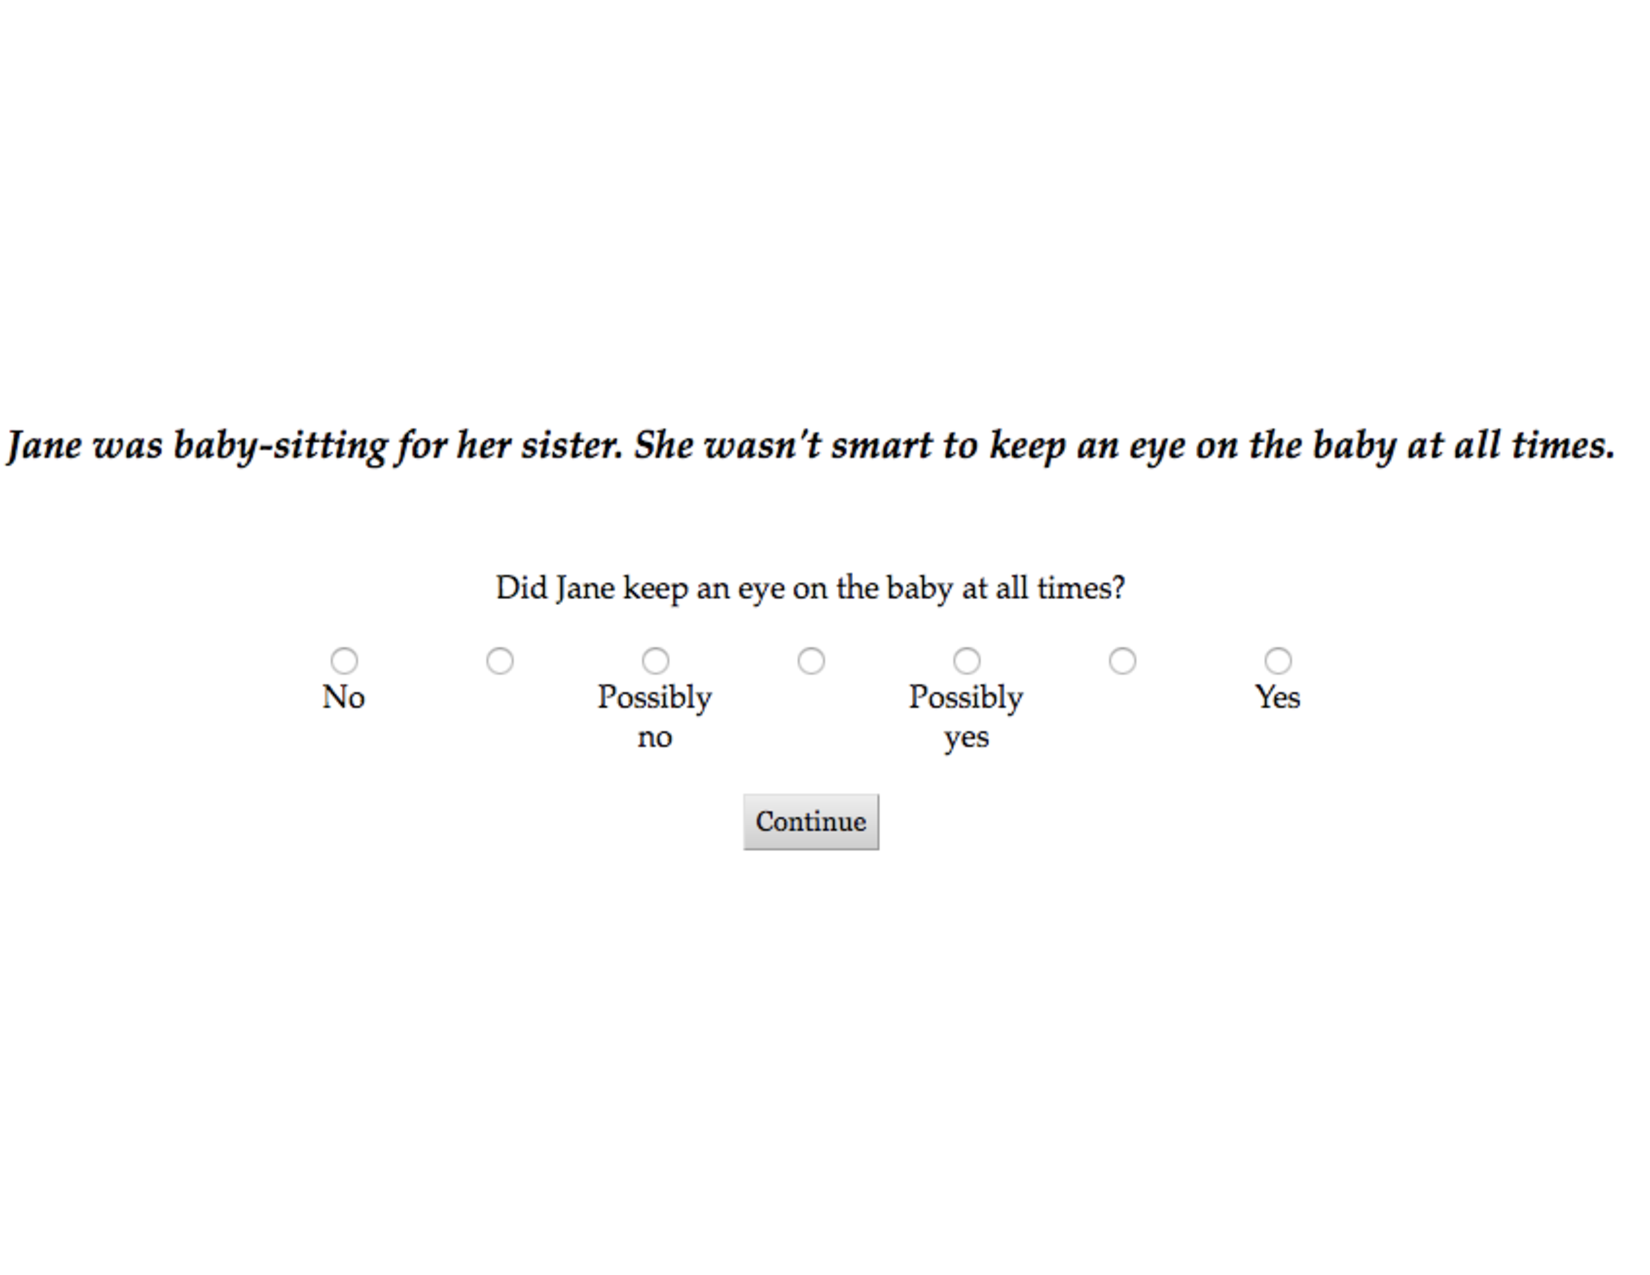
\includegraphics[width=.7\paperwidth]{figures/trial-exp1}}

\caption{A sample trial in Experiment 2}\label{f-trial-exp1}
\end{figure}

After rating the 16 stimuli, participants completed a brief questionnaire about their age, their
native language(s) and, if English is a native language, whether it is
American English, as opposed to e.g., Indian or Australian English.
Participants were told that they would be paid no matter how they
responded to these questions, in order to encourage them to answer
truthfully.


\paragraph{Data exclusion} The ratings from 5 participants who did not self-identify as native speakers of American English were excluded. 13 participants gave a response lower than 5/possibly yes to the control stimuli in (\ref{control-exp1}a-c) or higher than 3/possibly no to the control stimuli in (\ref{control-exp1}d-f). The ratings from these participants were also excluded, leaving data from 134 participants (ages: 18-69; mean age: 33).

\subsubsection{Results and discussion}

Each of the 120 target stimuli received between 9 and 14 ratings (mean: 11.2). As expected, the prejacents were more projective when the negation of the generalization follows from the common ground than when the generalization follows from the common ground: in the Content condition, the mean certainty ratings were 5.2 and 2.6, respectively; in the Context condition, the mean certainty ratings were 4.7 and 2.9, respectively. Figure \ref{f-condis}, which shows the mean projectivity ratings of the prejacents in the two conditions for each evaluative adjective, suggests that there is by-adjective variation in the projectivity of the prejacent and the influence of the discourse status of the generalization on the projectivity of the prejacent.

\begin{figure}[H]
\begin{center}
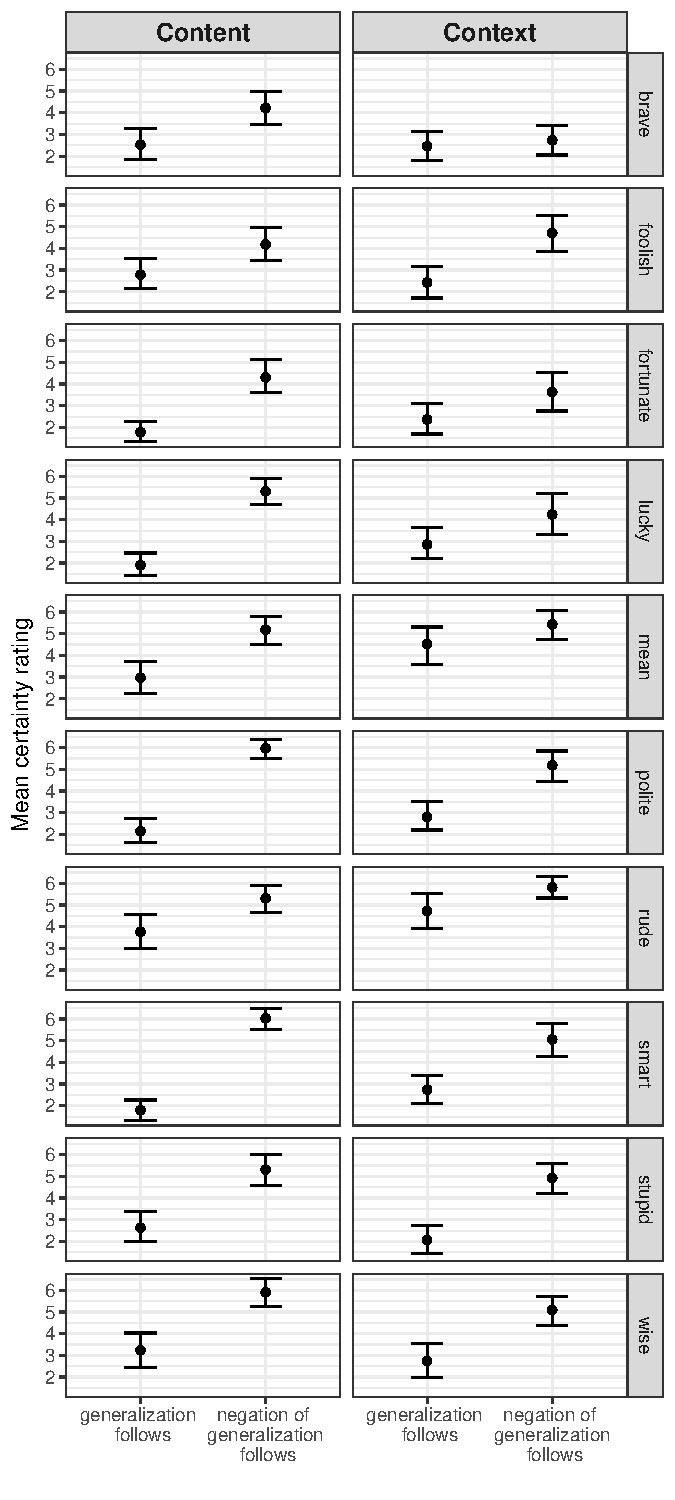
\includegraphics[scale=.7]{../exp2-projection/graphs/targetmeans-by-condition-and-adj}

\caption{Mean projectivity rating for prejacents of NEAS with the 10 evaluative adjectives in the Content condition (left panels) and the Context condition (right panels) by whether the generalization or its negation follow from the common ground. Error bars indicate bootstrapped 95\% confidence intervals.}\label{f-condis}
\end{center}
\end{figure}

We fitted ordinal mixed-effects regression models to the target data in the Content and Context conditions (668 and 672 data points, respectively), using the {\tt clmm} function of the {\tt ordinal} package (\citealt{Christensen2013}) in {\em R} (\citealt{r}; version 3.2.0). The models predicted projectivity ratings on the 7-point Likert scale from the fixed effect of the discourse status of the generalization (with `generalization follows' as the reference level). The models included the maximal random effects structure justified by the data and the theoretical assumptions: random by-participant intercepts (capturing differences in projectivity between participants), random by-adjective intercepts (capturing differences in projectivity between evaluative adjectives) and random by-item intercepts (capturing differences in projectivity between context/adjective/{\em to-}infinitive combinations) as well as random slopes for the discourse status of the generalization by participant and adjective (capturing that the effect of the discourse status may vary across participants and adjectives). We obtained $p$-values by comparing models via likelihood ratio tests.

There was a significant main effect of the discourse status of the generalization such that items in which the negation of the generalization follows received higher projectivity ratings in the Content ($\beta$ = 3.32, $SE$ = 0.35, $z$ = 9.5, $LR(1)$ = 27.11, $p <$ .001) and Context ($\beta$ = 2.04, $SE$ = 0.36, $z$ = 5.72, $LR(1)$ = 16.14, $p <$ .001) conditions. These findings suggest that the discourse status of the generalization influences projectivity, as predicted by the analysis developed in section \ref{s3}: prejacents of NEASs in which the negation of the generalization follows from the common ground are more projective than prejacents of NEASs in which the generalization follows from the common ground. These findings also suggest that readers attend both to information from the EAS and to information from the context in determining the extent to which the generalization follows from the common ground and, therefore, the extent to which the prejacent projects.

\subsection{Experiment 3: At-issueness of the prejacent}\label{s43}

This experiment tested the prediction in (\ref{pred}c): the stronger the inference to the truth of the generalization from the common ground, the more at-issue the prejacent is. The at-issueness diagnostic used in Exp.~3 relies on the assumption that at-issue and not-at-issue content differ in the extent to which it is up for debate and can be directly assented/dissented with. For previous uses of diagnostics that rely on this assumption see, e.g., \citealt{amaral-etal07,xue-onea11,murray2014,anderbois-etal2015,destruel-etal2015,tonhauser-sula6} and \citealt{syrett-koev2015}. The diagnostic we use here is the same as that in \citepos{tbd-variability} Exps.~2. The 3-turn dialogue in (\ref{sure}) illustrates how the diagnostic was set up on the basis of the appositive content associated with nominal appositives. The speaker of the first turn, Debby, utters an indicative sentence with the target expression, here a nominal appositive, and thereby commits herself to various utterance contents, including the appositive content that Martha's new car is a BMW. The speaker of the second turn, Harry, utters the question {\em Are you sure?}, thereby challenging some content of Debby's utterance. In the third turn, Debby utters an indicative sentence in which the content to be diagnosed for at-issueness, here the appositive content of her first utterance, realizes the content of the clausal complement of {\em sure}, thereby identifying it as the content that Debby took the Harry to be challenging. 

\begin{exe}
\ex\label{sure} At-issueness diagnostic from \citealt{tbd-variability}
\begin{xlist}
\exi{Debby:} Martha's new car, a BMW, was expensive.

\exi{Harry:} Are you sure?

\exi{Debby:} Yes, I am sure that Martha's new car is a BMW. 
\end{xlist}
\end{exe}

To assess whether the relevant content is up for debate, i.e., at-issue, participants were asked whether Debby's utterance answered Harry's question. A `yes' response was taken to indicate that the relevant content was at-issue: the content was targeted by Harry's question and, therefore, Debby answered Harry's question. A `no' response, in turn, was taken to indicate that the relevant content was not at-issue: the content was not targeted by Harry's question and, therefore, Debby did not answer Harry's question. We assume that the more at-issue a content is, the more `yes' responses it receives.

\subsubsection{Methods}

\paragraph{Participants} 75 participants, with US IP addresses and at least 97\% of HITs approved, were recruited on Amazon's Mechanical Turk platform (18-66, mean: 35). They were paid 35 cents.

\paragraph{Materials} Stimuli consisted of 3-turn discourses between Debby and Harry, as (\ref{sure2}) and (\ref{sure22}). In the target stimuli, the first turn of each discourse consisted of a past tense EAS that realized one of the 10 evaluative adjectives explored in Exp.~2. The second turn of the target stimuli consisted of Harry asking {\em Are you sure?}. In the third turn, Debby uttered {\em Yes, I am sure that}, with the prejacent of the EAS realized as the content of the finite complement of {\em sure that}. There were 6 sentences for each of the 10 evaluative adjectives, for a total of 60 target stimuli. Of the 6 sentences for each evaluative adjective, the generalization of 3 followed from the common ground, as in (\ref{sure2}); for the other 3 sentences, neither the generalization nor its negation followed from the common ground, i.e., the generalization was neutral, as in (\ref{sure22}). Participants were asked whether Debby answered Harry's question: a `yes' response was taken to indicate that Harry's question targeted the prejacent, i.e., the prejacent of Debby's utterance was taken to be at-issue, and a `no' response was taken to indicate that Harry's question did not target the prejacent, i.e., the prejacent of Debby's utterance was not taken to be at-issue. Given the analysis developed in section \ref{s3}, we expect the prejacent of EASs whose generalization follows from the common ground to be more at-issue, i.e., to receive more positive responses, than the prejacent of EASs with a neutral generalization. The full set of 60 target stimuli is provided in Appendix \ref{a-Exp2}.

\begin{exe}
\ex\label{sure2} Generalization follows from the common ground
\begin{xlist}
\exi{Debby:} Jane was stupid to post her social security number on Facebook. 

\exi{Harry:} Are you sure?

\exi{Debby:} Yes, I am sure that Jane posted her social security number on Facebook.
\end{xlist}

\ex\label{sure22} Neutral generalization
\begin{xlist}
\exi{Debby:} Jane was stupid to dance like that. 

\exi{Harry:} Are you sure?

\exi{Debby:} Yes, I am sure that Jane danced like that.
\end{xlist}
\end{exe}

The 60 target stimuli were distributed across 6 lists so that each of the 10 adjectives occurred once per list and each list had 5 target stimuli for which the generalization followed from the common ground and 5 target stimuli with a neutral generalization. To assess whether participants were attending to the task, each list also included the same two control stimuli shown in (\ref{control}): here, the main clause contents of Debby's first turns are assessed for at-issueness. These contents are hypothesized to be highly at-issue. 

\begin{exe}
\ex\label{control} Main clause control stimuli
\begin{xlist}
\ex
\begin{xlist}
\exi{Debby:} Mary brought a fruit salad.

\exi{Harry:} Are you sure?

\exi{Debby:} Yes, I am sure that Mary brought a fruit salad.
\end{xlist}
\ex 
\begin{xlist}
\exi{Debby:} Phillip, a yoga teacher, is wearing sweat pants.

\exi{Harry:} Are you sure?

\exi{Debby:} Yes, I am sure that Phillip is wearing sweat pants.
\end{xlist}
\end{xlist}
\end{exe}

Finally, to be able to compare the at-issueness of the prejacent to the at-issueness of other projective content, the same four control stimuli were added to each list. As shown in (\ref{proj}), these four control stimuli assessed the at-issueness of the content of a nominal appositive, of the possession implication of a possessive noun phrase, of the content of the clausal complement of the emotive predicate {\em be annoyed} and of the content of the clausal complement of the cognitive change-of-state predicate {\em discover}. In sum, each of the 6 lists consisted of 16 stimuli.

\begin{exe}
\ex\label{proj} Projective content control stimuli

\begin{xlist}

\ex Nominal appositive
\begin{xlist}
\exi{Debby:} Sue, a teacher, runs three times a week.

\exi{Harry:} Are you sure?

\exi{Debby:} Yes, I am sure that Sue is a teacher.
\end{xlist}


\ex Possessive noun phrase
\begin{xlist}
\exi{Debby:} Larry is flirting with your neighbor.

\exi{Harry:} Are you sure?

\exi{Debby:} Yes, I am sure that you have a neighbor.
\end{xlist}

\ex Emotive predicate {\em be annoyed} 
\begin{xlist}
\exi{Debby:} Tamara is annoyed that the pizza is gone.

\exi{Harry:} Are you sure?

\exi{Debby:} Yes, I am sure that the pizza is gone.
\end{xlist}

\ex Cognitive change-of-state predicate {\em discover}
\begin{xlist}
\exi{Debby:} Paula discovered that her husband is cheating.

\exi{Harry:} Are you sure?

\exi{Debby:} Yes, I am sure that Paula's husband is cheating.
\end{xlist}
\end{xlist}
\end{exe}

\paragraph{Procedure} 

Participants were told that they were at a party and that, upon walking into the kitchen, they overhear a short dialogue between Debby, the party host, and another guest, Harry. They were randomly assigned to a list and presented with the 16 stimuli, one after the other, in random order. They gave their ratings to the question of whether Debby answered Harry's question with two radio buttons labeled `yes' and `no', as shown in Figure \ref{f-trial-exp2}.  

\begin{figure}[H]
\centering

\fbox{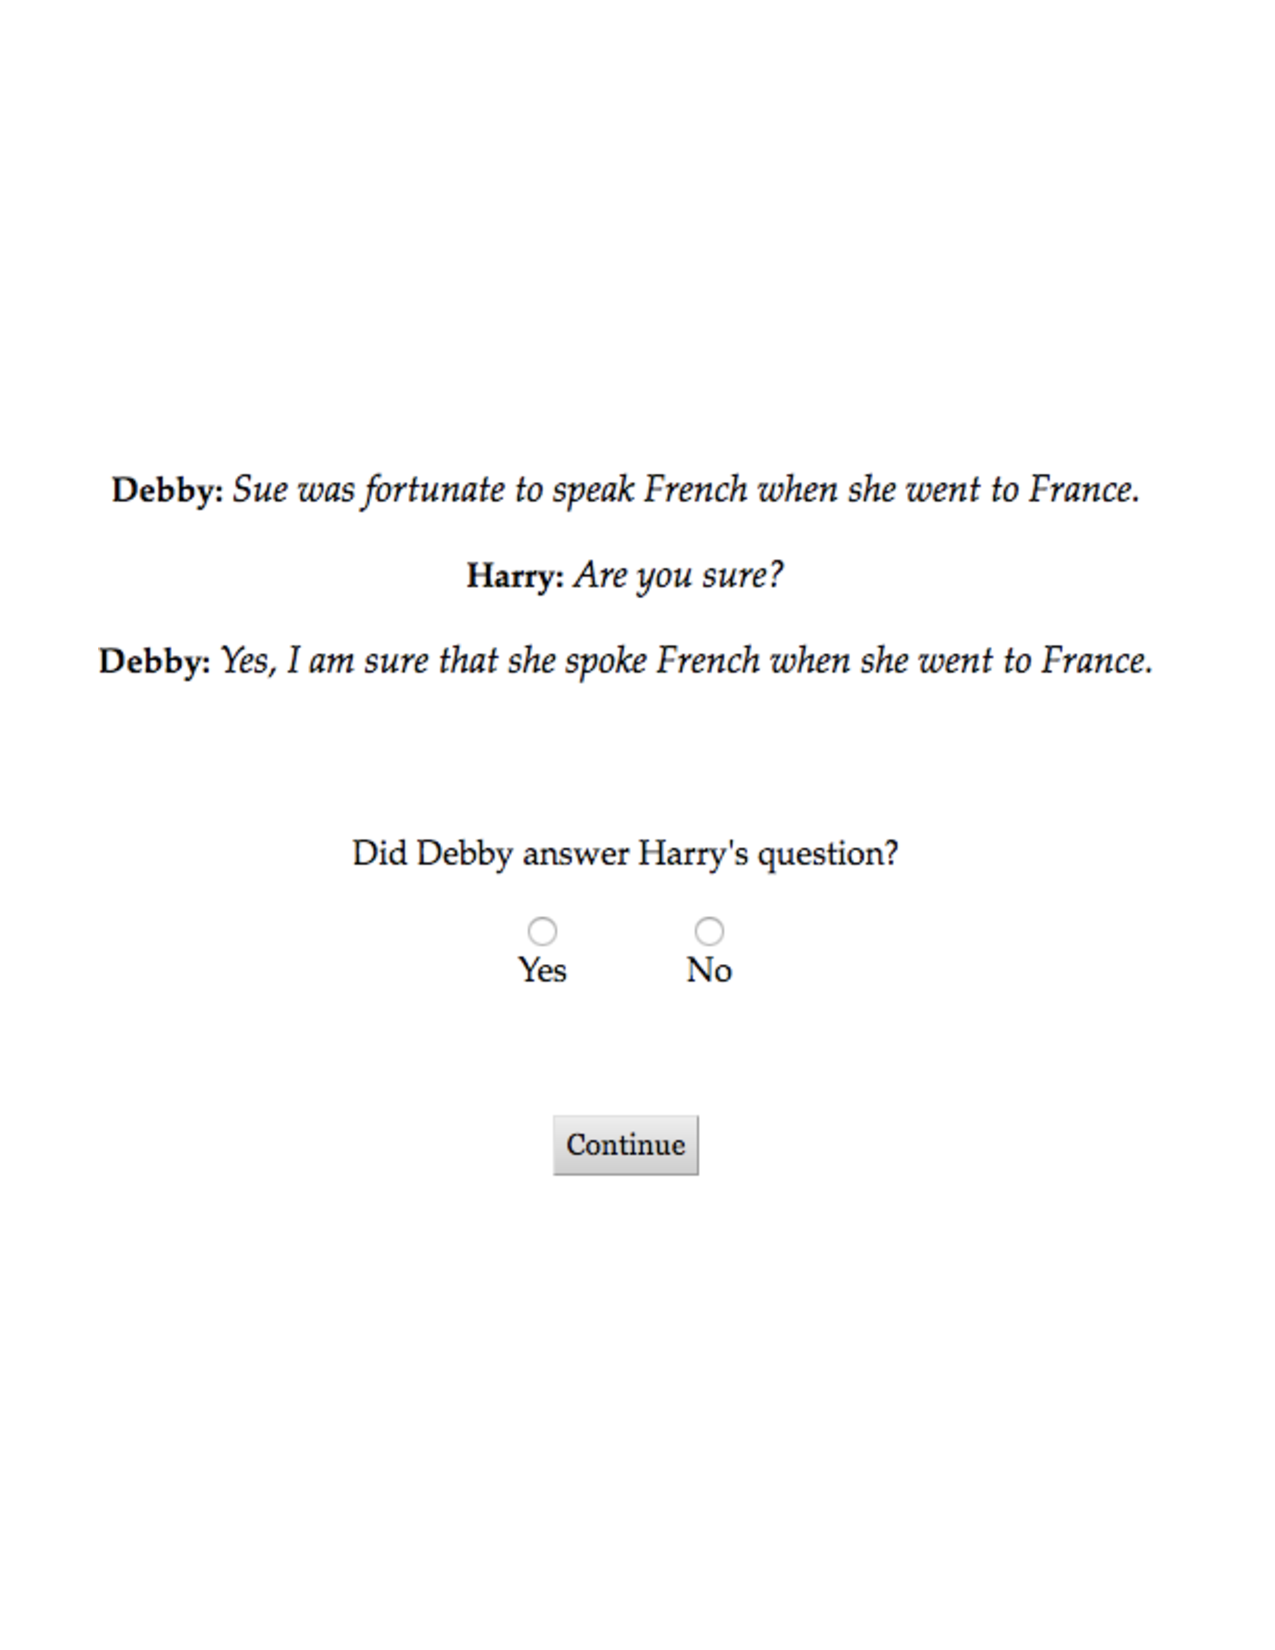
\includegraphics[width=10cm]{figures/trial-exp2}}

\caption{A sample trial in Experiment 3}\label{f-trial-exp2}
\end{figure}

After rating the 16 stimuli, participants filled out a brief questionnaire about their age, their native language(s) and, if English is a native language, whether it is
American English, as opposed to e.g., Indian or Australian English.
Participants were told that they would be paid no matter how they
responded to these questions, in order to encourage them to answer
truthfully.

\paragraph{Data exclusion} The ratings from 2 participants who did not self-identify as native speakers of American English were excluded. 5 participants answered `no' to one or both of the main clause control stimuli. The ratings from these participants were excluded, leaving data from 68 participants (ages: 18-66; mean: 35).

\subsubsection{Results and discussion}

Each of the 60 target stimuli received between 10 and 14 ratings (mean: 11.3).  Figure \ref{f-ai-by-adj} shows the proportion of `yes' responses, indicating at-issueness, in the two conditions:  as expected, prejacents of EASs whose generalizations follows from the common ground  received more `yes' responses than prejacents of EASs with neutral generalizations. This finding suggests that prejacents of EASs whose the generalizations follow from the common ground are more at-issue than prejacents of EASs with neutral generalizations, as predicted by the analysis developed in section \ref{s3}. As shown by the overlaid adjective means in Figure \ref{f-ai-by-adj}, the effect of the discourse status of the generalization was observed for all of the adjectives except {\em brave}.

\begin{figure}[H]
\begin{center}
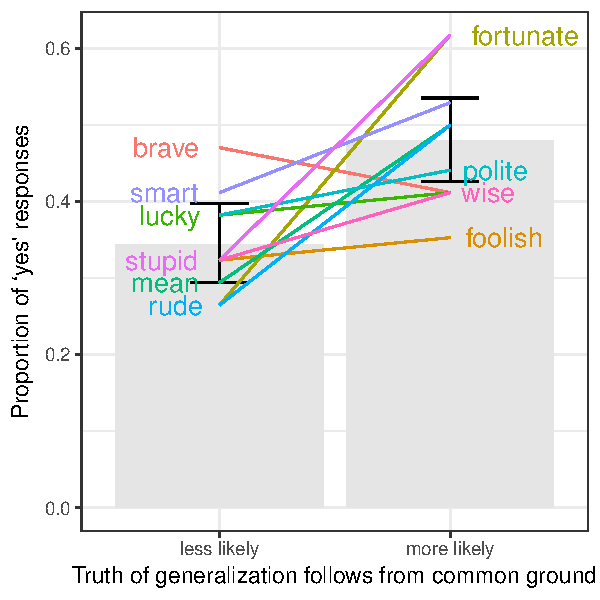
\includegraphics[scale=.85]{../exp3-at-issueness/graphs/proportion-ai-by-condition}

\caption{Proportion of `yes' responses, indicating at-issueness, by condition. Error bars indicate bootstrapped 95\% confidence intervals. Adjective means in the two conditions overlaid.}\label{f-ai-by-adj}
\end{center}
\end{figure}

To evaluate the effect of the discourse status of the generalization on the at-issueness of the prejacent, we fit a Bayesian binomial mixed effects model with uninformative priors using the R package \verb|brms| \citep{buerkner2017}.\footnote{We fit a Bayesian binomial mixed effects model rather than a \jt{regular?} one because \jt{reasons}. In fact, when we fit binomial mixed effects models, predicting response from a fixed effect of the discourse status of the generalizations, the models only converged if we included either a random by-adjective intercept or a random by-participant intercept, but not both. } The model predicted the log odds of `yes' over `no' ratings from a fixed effect of the discourse status of the generalization (with `neutral generalization' as the reference level). We included the maximal random effects structure justified by the design: random intercepts for item (capturing random differences in projectivity between items) and participant (capturing random differences in projectivity between participants) as well as random by-participant slopes for discourse status (capturing that the effect of discourse status may vary by participant). Four chains converged after 2000 iterations each (warmup = 1000, \(\hat{R}=1\) for all estimated parameters).

The model provided evidence for the predicted effect of the discourse status of the generalization on the at-issueness of the prejacent, such that  prejacents of EASs with generalizations that follow from the common ground were more likely to receive a `yes' rating than prejacents of EASs with neutral generalizations  ($\beta$ = 1.29, 95\% Credible Interval={[}0.69,1.87{]}).\footnote{In Bayesian mixed effects regression modeling, 95\% credible intervals indicate the range within which we can be certain with probability 0.95 that the parameter estimate $\beta$  lies, given the data at hand and our model (see, for example, Jaynes \& Kempthorne,1976;  Morey, Hoekstra, Rouder, Lee, \& Wagenmakers, 2016).\jd{JT, I'm unsure about how much info to include here and will add citations depending on what we decide to include}} This finding suggests that the prejacent of EASs with generalizations that follow from the common ground are more at-issue than that of EASs with neutral generalizations. 
%We fitted a binomial mixed-effects logistic regression predicting rating (0/no, 1/yes) from a fixed effect of condition (with EAS$_{\mbox{n}}$ as the reference level; 680 data points). The model included the maximal random effects structure justified by the data that allowed the model to converge: random by-adjective intercepts (capturing differences in at-issueness between adjectives).\footnote{A model that predicted rating from condition with a random by-participant intercept (capturing differences in at-issueness rating between participants) also revealed a main effect of condition ($\beta$ = 1.23, $SE$ = 0.23, $z$ = 5.32, $\chi^2$(1) = 27.62, $p <$ .0001).} The analysis was conducted using the lme4 package (\citealt{bates-etal2015}). A log-likelihood comparison of the model with the fixed effect to the model without the fixed effect revealed a significant main effect of EAS type. Specifically, the prejacent of EAS$_{\mbox{f}}$ received more `yes' ratings than the prejacent of EAS$_{\mbox{n}}$ ($\beta$ = 0.56, $SE$ = 0.16, $z$ = 3.57, $\chi^2$(1) = 12.89, $p =$ .0003), indicating that the prejacent of EAS$_{\mbox{f}}$ was judged to be more at-issue than that of EAS$_{\mbox{n}}$. 
These findings provide empirical support for the analysis developed in section \ref{s3}, which predicts that the prejacent of EASs is more likely to be at-issue when the generalization follows from the common ground than when it does not.\footnote{The projective content of the four control stimuli in (\ref{proj}) differed in the extent to which they received `no' ratings (indicating not-at-issueness): 94\% (64 of 68) for the appositive content in (\ref{proj}a), 90\% (61 of 68 for the possession content in (\ref{proj}b), 75\% (51 of 68) for the content of the clausal complement of {\em be annoyed} in (\ref{proj}c) and 44\% (30 of 68) for the content of the clausal complement of {\em discover} in (\ref{proj}d). We can compare these findings with the findings reported for similar contents in \citealt{tbd-variability}, whose Exp.~2a used the same diagnostic for at-issueness, but participants gave ratings on a slider. Further differences between the two experiments is that \citealt{tbd-variability} included more than one item for each of the projective contents but only included EASs with {\em stupid}. With these caveats in mind, we can note a similarity in the findings of the two experiments: as in the experiment reported on here, \citet{tbd-variability} found that the possession content and appositive content were most not-at-issue (mean ratings of .83 and .82, respectively), followed by the content of the clausal complement of {\em be annoyed} (mean: .78) and the prejacent of EASs (mean: .7), and finally the content of the clausal complement of {\em discover} (mean .47). These findings provide further support for the hypothesis that the prejacent of EASs overall is not highly not-at-issue.}


% Exp 2a Tonhauser, Beaver & Degen (Journal of Semantics)
%1        annoyed 0.77605042
%2       discover 0.47327731
%5         NomApp 0.81537815
%8         possNP 0.82810924
%10        stupid 0.69680672

% Exp2 here
%                    0          1
%  be_annoyed 0.75000000 0.25000000
%  discover   0.44117647 0.55882353
%  NomApp     0.94117647 0.05882353
%  possNP     0.89705882 0.10294118
%  EAS_n      0.65588235 0.34411765
%  EAS_f      0.52058824 0.47941176
  
\subsection{Summary and discussion}

According to the analysis of EASs developed in section \ref{s3}, the prejacent is not a lexically-specified presupposition but is projective in any given utterance to the extent that it is not at-issue with respect to the Discourse Question of the utterance. In this section, we explored the three predictions of the analysis given in (\ref{pred}) and repeated below for convenience:

\begin{exe}
\exi{(\ref{pred})} Predictions of the analysis for utterances of EASs

\begin{xlist}

\ex The projectivity of the prejacent is influenced by the focus marking of the utterance.

\ex The stronger the inference to the truth of the generalization from the common ground, the lower the projectivity of the prejacent.

\ex The stronger the inference to the truth of the generalization from the common ground, the higher the at-issueness of the prejacent. 

\end{xlist}
\end{exe}
All three predictions were borne out in the data. In section \ref{s41}, we provided tentative evidence from naturally occurring examples of NEASs for the prediction in (\ref{pred}a), by showing that what is focused influences whether the prejacent projects. In sections \ref{s42} and \ref{s43}, we provided experimental evidence for the predictions in (\ref{pred}b) and (\ref{pred}c), respectively. Specifically, the discourse status of the generalization was revealed to influence, in Exp.~2, the projectivity of the prejacent and, in Exp.~3, the at-issueness of the prejacent. 

\section{Two open issues}\label{s5}

Before concluding, we return to two issues that were raised in the introduction. The first issue is the status of the implication which we called the evaluation. As noted, while some authors consider this an entailment of EASs, we argue that it is merely an inference that arises from the prejacent and the generalization: in (\ref{f}), for instance, the prejacent (that Feynman danced on the table) and the generalization (that in dancing on the table Feynman is/would be stupid) jointly imply the evaluation, that Feynman dancing on the table was stupid. 

\begin{exe} 
\exi{(\ref{f})} Feynman was stupid to dance on the table. \hfill (\citealt[18]{barker02})

\end{exe} 
We also noted in section \ref{s1} that this inference exhibits a behavior that does not accord with it being a lexical entailment: it is negated in utterances of NEASs in which the prejacent projects but counterfactual when the prejacent doesn't project. The varying nature of the evaluation falls out straightforwardly from our analysis according to which it is not a lexical entailment. Consider first the NEAS in  (\ref{f2}a), repeated below: the speaker is taken to be committed to the prejacent (that Feynman danced on the table) and to the proposition that Feynman dancing on the table is not stupid. What follows is that the actual event of Feynman dancing on the table was not stupid. Now consider (\ref{nat}b), also repeated below, in which the prejacent does not project and the generalization follows from the common ground, i.e., is not negated. Here, the speaker is taken to be committed to the proposition that them stumbling through a junkyard in the dark is stupid and to the proposition that they did not stumble through the junkyard in the dark. What follows is a counterfactual inference, that the unrealized event of them stumbling through the junkyard in the dark is stupid, i.e., that them stumbling through the junkyard in the dark would be stupid. Thus, by not analyzing the evaluation as a lexical entailment, contrary to, e.g., \citealt{barker02}, our analysis correctly predicts the varying nature of the evaluation.

\begin{exe}
\exi{(\ref{f2}a)} Feynman wasn't stupid to dance on the table. \hfill (\citealt[18f.]{barker02})

\exi{(\ref{nat}b)} Now I knew someone was in the junkyard and the cold wind was
carrying the cries. I wasn't stupid to go stumbling through the
junkyard in the dark and get hurt. \hfill (\citealt[235]{karttunen-etal2014})

\end{exe}

Consider now the examples in (\ref{ant}), in which EASs occur in the antecedents of conditionals. In (\ref{ant}a), the prejacent projects, i.e., the speaker is taken to be committed to `Doggard escaped a German submarine attack'. The generalization restricts the conditional and so the speaker considers it a possibility that in escaping a German submarine attack Doggard is/would be lucky. Given that the speaker is committed to an actual, past event of Doggard escaping a German submarine attack, the speaker of (\ref{ant}a) is taken to be committed to the possibility that the actual, past event of Doggard escaping a German submarine attack was lucky. In (\ref{ant}b), the generalization, that anybody leaving the SAM running on Killing Floor is stupid, follows from the common ground of the interlocutors, i.e., the speaker is committed to it. The prejacent, that somebody left SAM running on Killing Floor, does not project but restricts the conditional. As a consequence, the speaker of (\ref{ant}b) is taken to be committed to the possibility that somebody did the stupid thing of leaving SAM running on the Killing Floor. In short, the evaluation of EASs embedded under other entailment-canceling operators differs from that of EAS embedded under negation.

\begin{exe}
\ex\label{ant} Embedding in antecedent of a conditional
\begin{xlist}

\ex If he [James Hamilton Doggart] was lucky to escape a German submarine attack in the Channel, he was even more fortunate to survive influenza, contracted while on leave in Cambridge.\footnote{\url{https://en.wikipedia.org/wiki/James_Hamilton_Doggart}}

%\ex If Feynman was stupid to dance on the table, then tell him. (= (\ref{f2}d)) \hfill (\citealt[18f.]{barker02})

\ex 
\begin{xlist}
\exi{A:} I wonder how many people would be banned for using SAM [Steam Achievement Manager] on Killing Floor.
\exi{B:} If they were stupid to leave it running then maybe a few.\footnote{\url{steamcommunity.com/app/730/discussions/0/540744934462316309/}}

\end{xlist} 
\end{xlist}
\end{exe}

What is considered a possibility also varies for EASs embedded under the possibility modal adverb {\em perhaps}, depending on whether the prejacent projects. In (\ref{perhaps}a), the prejacent projects and what is considered a possibility is the generalization: it is possible that us living in the times that we actually live in is lucky.  \jt{In this case, the evaluation is simply the present tense version of the the generalization, so the speaker conveys that the evaluation is possible. At any rate, some sentence that specifies the status of the evaluation} In (\ref{perhaps}b), on the other hand, the prejacent does not project and the speaker is taken to be committed to the generalization, that seeing the Northern Lights is lucky. Thus, the speaker of (\ref{perhaps}) considers it a possibility that they will participate in the for them lucky event of seeing the Northern Lights. 

\begin{exe}
\ex\label{perhaps}

\begin{xlist}

\ex Of course with the technology we possess today, electronic money is commonplace. [...] perhaps we are lucky to live in the times that we do.\footnote{\url{nrich.maths.org/2587}}

\ex I am seaching [sic] for a remote cabine in Finland that is available for renting. [...]
Region wise I would prefer Lapland or Lakeside. Perhaps we are lucky to see northern lights.\footnote{\url{www.tripadvisor.com/ShowTopic-g189896-i442-k11448709-Remote_rental_cottage-Finland.html}}

\end{xlist}

\end{exe}
In sum, the evaluations of utterances of EASs differ depending on i) whether they are embedded under entailment-canceling operators, ii) which entailment-canceling operator they are embedded under and iii) whether the prejacent projects. The varying nature of the evaluation falls out from our analysis according to which EASs lexically entail the prejacent and the generalization. 

The preceding discussion has also highlighted an aspect of the interpretation of utterances of EAS that differs from the interpretation of utterances of other sentences that give rise to projective content, namely the complementary behavior of the prejacent and the generalization: when the prejacent projects, the generalization does not, and when the prejacent does not project, the generalization does. That this behavior is strikingly different from the interpretation of utterances of other sentences that give rise to projective content is illustrated with the example in (\ref{stop}). When the content of the clausal complement of {\em know} (that the meeting was canceled) projects, what is denied is Sam's knowledge of this proposition. The critical difference between EAS and examples like (\ref{stop}) comes out when the content of the clausal complement does not project (as is brought out, for instance, by the continuation {\em \ldots he, like all of us, is in the dark about whether the meeting will take place}). In this case, Sam's knowledge of the proposition that the meeting was canceled is still denied and the speaker is not taken to be committed to either the truth or the falsity of the content of the clausal complement. 

\begin{exe}
\ex\label{stop} Sam doesn't know that the meeting was canceled.
\end{exe}
This observation has strong implications for analyses of EAS according to which the prejacent is a lexically-secified presupposition. First, when the prejacent is locally accommodated under negation, the speaker is committed to the falsity of the prejacent; this is in contrast to a locally accommodated factive presupposition, for which the speaker is not committed to its truth or falsity. Second, when the prejacent is locally accommodated under some operator, the generalization is not interpreted under that operator, in contrast to the attitude ascription with {\em know} which is always interpreted in the scope of the operator. These observations are problematic for advocates of an account of EAS in which the prejacent is treated as a lexically-specified presupposition and projection is assumed to be governed by the standard mechanisms of presupposition projection (\citealt{heim83,vds92}).

%\begin{exe}
%\ex\label{qu} Embedding under polar question operator
%
%\begin{xlist}
%
%\ex A man, aged 20, [...] smoked weed with his friends at Thanksgiving. [...] Was he \fbox{foolish} to have smoked the weed [...]?\footnote{\url{https://community.babycentre.co.uk/post/a30729499/taken_off_transplant_list_for_smoking_weed}}
%
%\ex {[}Endredi:] ``Do you mean people sell false relics?'' \\ ``All the time,'' Adelar said. ``To those foolish enough to trust whatever they are told.'' \\ Endredi did not reply. It was appalling, of course, to think that anyone would seek to profit by such a fraud. However, she was also struggling not to attach any significance to Adelar's words. She kept thinking he was speaking in riddles. For instance, was she foolish to trust his words long ago? Was she \fbox{foolish} to trust him now? [...] She was not anxious to spend more time in Adelar's company than she had to. \hfill (Margaret Moore, {\em The Saxon})
%
%%\ex The `intellectualist' (Ryle's opponents) would argue against this by saying that he never really or fully knew the truths about the game that the grandmaster was imparting, but Ryle argues that, if the novice were stupid, then a) he would not be able to recall the appropriate rule at the time of making the move, and b) even if he did recall the appropriate rule, he might be \fbox{stupid} to follow it.
%%
%%\url{philosophymasters.wordpress.com/2012/01/15/reading-gilbert-ryle-knowing-how-and-knowing-that/}
%
%\end{xlist}
%
%\end{exe}

\jt{Also talk about hypothesis that some people don't like prejacent to be at-issue}

The second issue we return to is the observation, made in section \ref{s1}, that not all native speakers of American English judge NEAS in which the prejacent does not project to be acceptable. What might this variation be due to? One hypothesis is that speakers differ in their lexical entries for evaluative adjectives. One way of specifying such a hypothesis is that a first group of speakers, those that judge NEAS in which the prejacent does not project to be acceptable (around 20-30\% of the population), have a lexical entry according to which the prejacent is not lexically specified as a presupposition (as in the analysis developed in section \ref{s3}), thereby allowing them to produce NEAS in which the prejacent projects or doesn't project. The second group of speakers, those that judge such NEAS to be unacceptable, have a lexical entry according to which the prejacent is lexically specified as a presupposition, thereby resulting in them preferring to produce NEAS in which the prejacent projects. When interpreting NEAS, speakers in the second group should consistently assign projecting interpretations to prejacents of NEAS in which the negation of the generalization follows from the common ground because the projecting interpretation is not only the lexically specified interpretation but also supported by  common ground information. A similar hypothesis can be found in \citet[243]{karttunen-etal2014}, who suggested that there are about 3 times as many speakers who prefer giving interpretations to NEAS in which the prejacent projects, using the lexical entry in (\ref{lex}a), than speakers who prefer giving interpretations to NEAS in which the prejacent doesn't project, using the lexical entry in (\ref{lex}b). Thus, both hypotheses lead to the expectation that a substantial number of native speakers of American English (about 70-80\%) consistently assign projecting interpretations to NEAS in which the negation of the generalization follows from the common ground.

A post-hoc analysis of the findings of Exp.~2 suggests that both hypotheses should be rejected. Recall that each participant in Exp.~2 rated the projectivity of the prejacent of NEAS on a 7-point Likert scale: they rated the projectivity of the prejacent of 5 NEAS in which the generalization follows from the common ground and of 5 NEAS for which the negation of the generalization follows from the common ground. To explore the aforementioned hypotheses, we calculated each participants' mean projectivity ratings for these two types of NEAS: these mean projectivity ratings are an indication of how projective participants rated the prejacent of the two types of NEAS. Under both hypotheses, we expect a majority of participants to assign highly projective interpretations to the prejacent of NEAS for which the negation of the generalization follows from the common ground. 

\jt{Mandy: I am getting really confused trying to wrap my head around this. (I thought I understood it last time...) Can you write this with some reminders about why we should expect reading X in case Y for participant of type Z? (if that makes sense...)}

The histogram in Figure \ref{f-dialect} shows the 134 participants' mean projectivity ratings for the two types of NEAS. The right panel reveals that, of the 134 participants, only 23 (17\%) had mean projectivity ratings of at least 6.5 for the NEAS in which the negation of the generalization follows from the common ground; when considering mean projectivity ratings of at least 5.5, this number still only rises to 55 (41\%) participants. Thus, we do not find that a majority of the 134 participants assigned highly projective interpretations to prejacents of NEAS for which the negation of the generalization follows from the common ground. This observation calls into question the hypothesis that a majority of native speakers of American English have a lexical entry for evaluative adjectives according to which the prejacent is a lexically-specified presupposition. 


\begin{figure}[h!]
\begin{center}
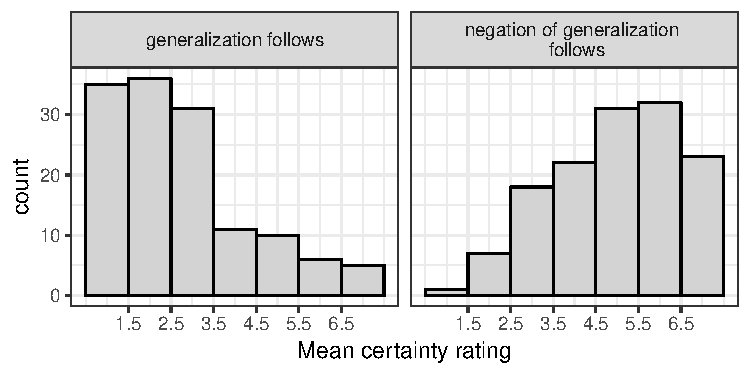
\includegraphics[scale=.9]{../exp2-projection/graphs/count-of-participants}

\caption{Participants' mean projectivity ratings for the two types of NEAS in Exp.~2}\label{f-dialect}
\end{center}
\end{figure}

We leave further explorations of the question of why native speakers of American English differ in their acceptability judgments for NEAS with non-projecting prejacents to future research.

\section{Conclusions}\label{s6}

This paper explored the projectivity of the prejacent of EASs. Contrary to the predictions of analyses of the prejacent as a lexically-specified presupposition (e.g., \citealt{barker02,oshima09b}), we showed, based on a corpus study of naturally occurring NEASs, that the prejacent is not highly projective (see also \citealt{tbd-variability}). According to the analysis we developed, the prejacent of an utterance of an EAS projects to the extent that it is not at-issue with respect to the Discourse Question addressed by the utterance. The Discourse Question, we showed, is constrained by the information-structural focus of utterances of EASs as well as by the discourse status of the generalization. Three predictions of the analysis were found to be empirically verified: i) the focus marking of naturally occurring NEASs differs depending on whether the prejacent projects, ii) the discourse status of the generalization influences the projectivity of the prejacent, and iii) the discourse status of the generalization influences the at-issueness of the prejacent. Our analysis, we argue, is more parsimonious than that of \citealt{karttunen-etal2014} according to which evaluative adjectives are systematically ambiguous.

The question-based analysis of the projectivity of the prejacent of EASs developed in this paper contributes to our understanding of how content comes to be projective without being conventionally specified as a presupposition or a conventional implicature. In its reliance on information-structural focus and the question-based organization of discourse, our analysis has strong parallels with \citepos{abrusan2013} and \citepos{stevens-etal2017} analyses of the projective content of manner adverb utterances (like {\em Did Martha run quickly?}) and with \citepos{best-question} analysis of the projective content of utterances with {\em know} (like {\em Does Martha know that Harry is having a party?}). We do not believe that these kinds of analyses are empirically adequate for any kind of projective content. We take, for instance, the requirement of the pronoun {\em she} that there be a uniquely salient antecedent discourse referent to be part of the conventionally coded content of the pronoun. Likewise, the projectivity of the appositive content of non-restrictive relative clauses may be best derived from a conventional specification of the discourse status of expressions (e.g., \citealt{potts05,murray2014}). Thus, one of the exciting challenges for future research on projective content is to identify, for any given projective content, whether its empirical properties warrant a non-lexical analysis of its projectivity. The empirical properties of the prejacent of EASs that were identified in this paper may provide guidance in this decision process.


\appendix

\section{Acceptability rating experiment}\label{s-acc}

The acceptability rating experiment was designed to explore the acceptability of  NEASs whose prejacent does not project. 

\subsection{Methods}

\paragraph{Participants} 134 participants with US IP addresses and at least 97\% of HITs approved were recruited on Amazon's Mechanical Turk platform (ages: 20-72; mean: 33). They were paid 45 cents.

\paragraph{Materials} Stimuli consisted of three-sentence discourses. In the target stimuli, the last sentence was either a NEAS, as in (\ref{jenny}a), or a variant of the NEAS in which the evaluative adjective was followed by {\em enough}, as in (\ref{jenny}b). The first two sentences of the discourses denied the truth of the prejacent of the third sentence to ensure that the prejacent of the third sentence could not project: in (\ref{jenny}), for instance, the first two sentences convey that Jenny left the baby unattended, which contradicts the prejacent, that Jenny kept an eye on the baby at all times. We hypothesized that participants would judge the NEAS to be acceptable only if they would realize an interpretation in which the prejacent projects with the NEAS. We further hypothesized that the variant with {\em enough} would be judged to be acceptable by all participants.

\begin{exe} 
\ex\label{jenny} 
\begin{xlist}
\ex Jenny was baby-sitting for her sister. She
left the baby unattended. \\ \underline{She wasn't smart to keep an eye on the baby at all times.} 

\ex Jenny was baby-sitting for her sister. She
left the baby unattended. \\ \underline{She wasn't smart enough to keep an eye on the baby at all times.} 

\end{xlist}
\end{exe} 

The target stimuli consisted of 6 pairs of three-sentence discourses like (\ref{jenny}) for each of the 10 evaluative adjectives explored in the experiments reported on in the main body of the paper, for a total of 60 pairs of target stimuli. The full set of target stimuli is provided in the GitHub repository mentioned in footnote \ref{f-git}. The 120 target stimuli were distributed across 12 lists of 10 each so that each adjective occurred only once per list, and each list included 5 NEASs and 5 variants with {\em enough}. 

To assess whether participants were paying attention to the task, the same 8 control stimuli were added to each list, for a total of 18 stimuli per list. The control stimuli consisted of three-sentence discourses in
which the last sentence contradicted the second one, as illustrated in
(\ref{claire}). We expected the last sentence of the control stimuli to be judged to be unacceptable as part of the discourse.

\begin{exe} 
\ex\label{claire} 
\begin{xlist}
\ex Claire fell down the stairs. She broke a leg and some ribs. \uline{She was glad to not be hurt.} 

\ex Earl had a bad toothache. He called his dentist. \uline{He forgot to call his dentist.}

\ex Ross was doing his laundry. He found coins in his pocket. \uline{He didn't manage to find coins anywhere.}

\ex Charles was on a date with Susanne. He was having a bad time. \uline{He was happy to be having a great time.}

\ex Keith was hiking up a steep mountain. He didn't make it to the top. \uline{He was ecstatic to have made it to the top.}

\ex Liv went on a trip to Europe. She spent a lot of time in Italy. \uline{She failed to visit Italy.}

\ex Fran lived in Paris. She shared an apartment with some friends. \uline{She wasn't sad to live alone.}

\ex Tess had failed many college classes. She didn't graduate. \uline{She was proud to have graduated from college.}

\end{xlist}
\end{exe}


\paragraph{Procedure} Participants were told that they would read descriptions of a scenario and asked to judge whether the last, underlined sentence sounds good as part of the description. They gave their ratings on a 7-point Likert scale
labeled at four points: No/1, Possibly no/3, Possibly yes/5,
Yes/7). Participants were randomly assigned to a list and presented with the 18 stimuli, one after the other, in a random order. After rating the 18 stimuli, participants filled out a brief questionnaire about their age, their native language(s) and, if English is a native language, whether it is American English, as opposed to e.g., Indian or Australian English.
Participants were told that they would be paid no matter how they
responded to these questions, in order to encourage them to answer
truthfully.


\paragraph{Data exclusion} 

The ratings from 2 participants who did not self-identify as native speakers of American English were excluded. 38 participants gave a rating higher than Possibly no/3 to one or more of the eight unacceptable control stimuli. The ratings from these participants were also excluded, leaving data from 94 participants (ages: 20-67; mean: 33). 

\subsection{Results}

As expected, target stimuli with {\em enough} were judged to be acceptable: the mean rating for such items was 5.9 and most ratings were 5 or higher (409 of 477 responses,
86\%). Ratings for the target stimuli with NEASs were lower, with a mean rating of 4.2. As shown in the left panel of Figure \ref{f-acc}, NEASs (abbreviated `NEAS') received lower ratings overall.

To identify whether a participant judged NEASs in which the prejacent does not project to be acceptable, we calculated each participants' mean rating of the 5 stimuli with a NEAS. We then subtracted this mean rating from their mean rating for the 5 stimuli with {\em enough}. The resulting `acceptability score' is a measure of how acceptable NEASs with non-projecting prejacents are compared to acceptable stimuli with {\em enough}. An acceptability score of 0 means that the participant judged the NEASs with non-projecting prejacents as acceptable as stimuli with {\em enough}. The right panel of Figure \ref{f-acc} plots the participants' acceptability scores; the red line indicates an acceptability score of 0. Of the 94 participants, 20 (21\%) had an acceptability score of at least 0 and 27 (29\%) had an acceptability score of at least -0.5. Thus, although there are also many participants who do not judge NEASs in which the prejacent does not project to be acceptable, a sizable portion of (self-reported) native speakers of American English judge such sentences to be acceptable.

\begin{figure}[h!]

\hspace*{-.5cm}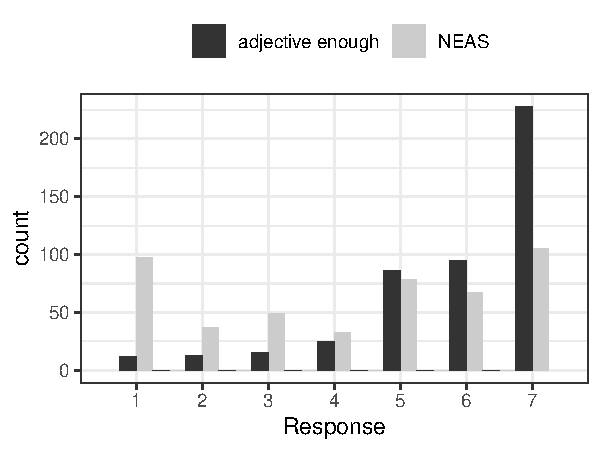
\includegraphics[scale=.8]{../acceptability-rating-study/graphs/histogram} 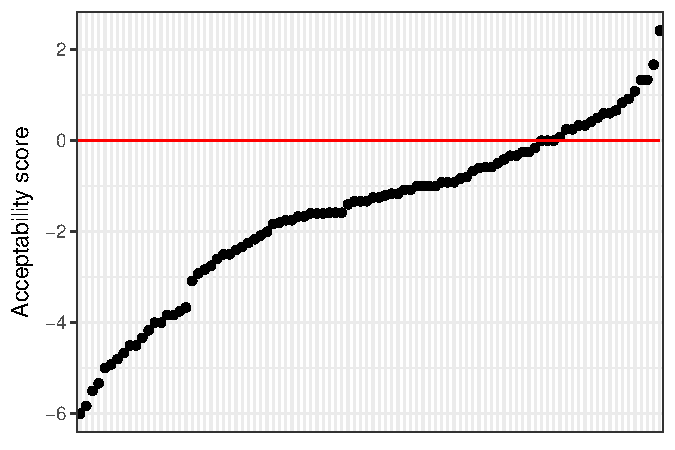
\includegraphics[scale=.8]{../acceptability-rating-study/graphs/acceptability-rating-difference}


\caption{Count of ratings of target stimuli (left panel) and acceptability scores of participants (right panel)}\label{f-acc}

\end{figure}

\section{Norming study for Exp.~1}\label{a-norming}

The goal of the norming study was to identify generalizations of EASs that follow from the common ground or whose negation follows from the common ground. 

\subsection{Methods}

\paragraph{Participants} 270 participants, with US IP addresses and at least 97\% of HITs approved, were recruited on Amazon's Mechanical Turk platform (ages 18-68, 1 undeclared; mean: 32). They were paid 45 cents.


\paragraph{Materials} For each of the ten evaluative adjectives of Exp.~1, we created 12 pairs of two-sentence stimuli such that the first sentence was a context sentence and the second sentence a NEAS, as in (\ref{cont}) and (\ref{context}). We hypothesized, for each pair of NEASs, that the generalization of one member of the pair follows from the common ground and the negation of the generalization of the other member of the pair follows from the common ground. Target stimuli in the norming study consisted of two-sentence discourses where the first sentence was the context sentence of the stimuli in Exp.~1 and the second sentence was the prejacent of the NEAS, as shown in (\ref{cont-norm}) and (\ref{context-norm}) for the stimuli in (\ref{cont}) and (\ref{context}), respectively. Given that there were 120 pairs of potential stimuli for Exp.~1, there were 120 pairs of two-sentence discourses in the norming study, i.e., a total of 240 two sentence discourses. The full set of target stimuli is provided in the GitHub repository mentioned in footnote \ref{f-git}. To assess whether the generalization or its negation follow from the common ground, participants were asked to assess the truth of the corresponding generalization. The generalizations were presented in the past tense to cohere with the tense of the discourses that participants read.


\begin{exe}
\ex\label{cont-norm} Sample stimuli in the Content condition 

\begin{xlist}
\ex Sue was traveling in France. She lost her wallet. \\ (Question to  participants: `Was Jane fortunate to lose her wallet?')

\ex Sue was traveling in France. She spoke some French. \\ (Question to participants: `Was Jane fortunate to speak French?')

\end{xlist}

\ex\label{context-norm} Sample stimuli in the Context condition

\begin{xlist}
\ex Jane was prank-calling people. She called the police. \\ (Question to participants: `Was Jane smart to call the police?')

\ex Jane saw a man with a gun. She called the police. \\ (Question to participants: `Was Jane smart to call the police?')
\end{xlist}
\end{exe}

The 240 target stimuli were distributed into 24 lists of 10 target stimuli so that each list included one target stimulus for each evaluative adjective. Each list included 5 target stimuli in which the generalization was hypothesized to follow from the common ground and 5 in which the negation of the generalization was hypothesized to follow from the common ground. Each list included 5 stimuli each from the target stimuli created for the Context and Content conditions.

To assess whether participants were attending to the task, the same 4 control stimuli were added to each list, for a total of 14 stimuli per list. The control stimuli consisted of two-sentence discourses, as shown in (\ref{controls-norming}): the two controls in (\ref{controls-norming}a-b) were expected to receive a positive answer and the two controls in (\ref{controls-norming}c-d) were expected to receive a negative answer.

\begin{exe}
\ex\label{controls-norming}
\begin{xlist}
\ex Earl worked in London last year. He was a teacher at a private school. 
\\ (Is it true that Earl worked at a private school in London?)

\ex Liv was having a birthday party. She bought a cake for her party.
\\ (Is it true that Liv bought a cake for her birthday party?)

\ex Claire was knitting a sweater. She was using red yarn. 
\\ (Is it true that Claire was knitting a blue sweater?)

\ex Ross graduated from college yesterday. He was an excellent student. 
\\ (Is it true that Ross dropped out of college?)

\end{xlist}
\end{exe}

\paragraph{Procedure}

Participants were told that they would read descriptions of a scenario and asked to respond to a question about the scenario. They gave their responses on a 7-point Likert scale labeled at four points: No/1, Possibly no/3, Possibly yes/5,
Yes/7). Participants were randomly assigned to a list and presented with the 14 stimuli, one after the other, in a random order. After rating the 14 stimuli, participants filled out a brief questionnaire about their age, their native language(s) and, if English is a native language, whether it is American English, as opposed to e.g., Indian or Australian English. Participants were told that they would be paid no matter how they
responded to these questions, in order to encourage them to answer
truthfully.


\paragraph{Data exclusion} 

The ratings from 9 participants who did not self-identify as native speakers of American English were excluded. 31 participants gave ratings lower than Possibly yes/5 to the control stimuli in (\ref{controls-norming}a-b), for which we expected the speaker to be taken to be committed to the relevant content, or higher than Possibly no/3 to the control stimuli in (\ref{controls-norming}c-d), for which we expected the speaker to not be taken to be committed to the relevant content. The ratings from these participants were also excluded, leaving data from 230 participants (ages: 18-68; mean: 32). 

\subsection{Analysis}

Each of the 240 target discourses received between 7 and 13 ratings (mean: 9.6). As shown in Table \ref{t-mean-norming1}, stimuli for which the generalization was hypothesized to follow generally received high ratings and stimuli for which the negation of the generalization was hypothesized to follow generally received low ratings.

\begin{table}[!h]
\centering

\begin{tabular}{l|cc}
& \multicolumn{2}{c}{What was hypothesized to follow:} \\
& generalization & negation of generalization \\\hline

Content condition &  6.2 (1.2) &  1.6 (1.1) \\
Context condition &  6.0 (1.3) &  2.2 (1.6) \\

\hline
\end{tabular}

\caption{Mean ratings and standard deviations for the 240 stimuli in the four conditions}\label{t-mean-norming1}

\end{table}

Of the 120 pairs of target stimuli (60 pairs in the Context and Content conditions each), we selected the 6 best pairs for each evaluative adjective: 3 in the Context condition and 3 in the Content condition: the `best' pairs of stimuli were those where the mean ratings of the two members of the pair were as high and low as possible, respectively. The mean ratings and standard deviations for the 120 stimuli selected for Exp.~1 are shown in Table \ref{t-mean-final}.

\begin{table}[!h]
\centering

\begin{tabular}{l|cc}
& \multicolumn{2}{c}{What was hypothesized to follow:} \\
& generalization & negation of generalization \\\hline

Content condition &  6.5 (0.9) &  1.3 (0.8) \\
Context condition &  6.1 (1.2) &  1.7 (1.2) \\

\hline
\end{tabular}

\caption{Mean ratings and standard deviations for the 120 selected stimuli in the four conditions}\label{t-mean-final}

\end{table}

%
%The best  pairs of stimuli in the content condition have the following
%properties: the mean for the consonant member of the pair is 5.75 or
%higher and the mean for the dissonant member of the pair is 2.1 or
%lower. The difference between the means of the pairs was 5.2 (sd: 0.5)).
%
%The best pairs of stimuli in the context condition have the following
%properties, with five exceptions, discussed below: the mean for the
%consonant member of the pair is 5.2 or higher and the mean for the
%dissonant member of the pair is 2.3 or lower. For three adjectives, we
%had to select pairs of less ideal stimuli (since no better stimuli were
%available), namely for {\em brave, lucky} (2 pairs each) and {\em mean} (1 pair). The difference between the means of the selected pairs was 4.4 (sd: 1).
%


\section{Materials of Exp.~1}\label{a-Exp1}

There were 12 stimuli for each of the 10 evaluative adjectives: 6 stimuli in the Content condition (Cn) and 6 in the Context condition (Cx). For stimuli marked whose coding ends with an `T' (i.e., [xxT]), the norming study established that the strength of the inference to the truth of the generalization from the common ground was high, i.e., the generalization follows from the common ground. For stimuli whose coding ends with an `F' (i.e., [xxF]), the norming study established that the strength of the inference to the falsity of the generalization was high.

\begin{itemize}[itemsep=-1pt]

\item {\bf brave}

\begin{enumerate}[topsep=0pt,itemsep=-4pt]

\item[CnT] 	Greg wrote a controversial article.	He	wasn't brave	to use his own name.
\item[CnT] 	Greg saw a child drowning in a river.	He	wasn't brave	to jump into the river.
\item[CnT] 	Greg saw a man hit a dog.	He	wasn't brave	to stand up to the man.
\item[CnF] 	Greg wrote a controversial article.	He	wasn't brave	to use a fake name.
\item[CnF] 	Greg saw a man hit a dog.	He	wasn't brave	to walk away.
\item[CnF] 	Greg saw a child drowning in a river.	He	wasn't brave	to watch from the river bank.
\item[CxT] 	Greg was being attacked by five men.	He	wasn't brave	to take them on.
\item[CxT] 	Greg was asked to speak up against the crime boss.	He	wasn't brave	to agree to do it.
\item[CxT] 	Greg was offered a job as a lion tamer.	He	wasn't brave	to take the job.
\item[CxF] 	Greg was asked to help his friend move.	He	wasn't brave	to agree to do it.
\item[CxF] 	Greg was asked to mow his neighbor's lawn.	He	wasn't brave	to take the job.
\item[CxF] 	Greg was being tickled by two small boys.	He	wasn't brave	to take them on.

\end{enumerate}

\item {\bf foolish}

\begin{enumerate}[topsep=0pt,itemsep=-4pt]


\item[CnT] 	Kate's doctor told her to lose weight.	She	wasn't foolish	to ignore him.
\item[CnT] 	Kate took her nephew to the playground.	She	wasn't foolish	to wear high heels.
\item[CnT] 	Kate was working a very stressful job.	She	wasn't foolish	to ignore her health problems.
\item[CnF] 	Kate's doctor told her to lose weight.	She	wasn't foolish	to start exercising.
\item[CnF] 	Kate took her nephew to the playground.	She	wasn't foolish	to bring water and a snack.
\item[CnF] 	Kate was working a very stressful job.	She	wasn't foolish	to take relaxation classes.
\item[CxT] 	Kate had a broken ankle.	She	wasn't foolish	to go for a run.
\item[CxT] 	Kate was completely broke.	She	wasn't foolish	to go shopping.
\item[CxT] 	Kate was drunk at a bar.	She	wasn't foolish	to take her top off.
\item[CxF] 	Kate needed a new dress.	She	wasn't foolish	to go shopping.
\item[CxF] 	Kate was getting a breast exam.	She	wasn't foolish	to take her top off.
\item[CxF] 	Kate wanted to exercise.	She	wasn't foolish	to go for a run.

\end{enumerate}

\item {\bf fortunate}

\begin{enumerate}[topsep=0pt,itemsep=-4pt]



\item[CnT] 	Sue was traveling in France.	She	wasn't fortunate	to speak some French.
\item[CnT] 	Sue was bitten by a shark.	She	wasn't fortunate	to get away with a few cuts.
\item[CnT] 	Sue was training to become a dancer.	She	wasn't fortunate	to have a great sense of rhythm.
\item[CnF] 	Sue was bitten by a shark.	She	wasn't fortunate	to lose a leg.
\item[CnF] 	Sue was traveling in France.	She	wasn't fortunate	to get robbed.
\item[CnF] 	Sue was training to become a dancer.	She	wasn't fortunate	to develop back problems.
\item[CxT] 	Sue needed to get some rest.	She	wasn't fortunate	to fall asleep.
\item[CxT] 	Sue spontaneously went to the beach.	She	wasn't fortunate	to be wearing flip-flops.
\item[CxT] 	Sue needed a present for her sick friend.	She	wasn't fortunate	to have a flower bouquet.
\item[CxF] 	Sue is allergic to pollen.	She	wasn't fortunate	to have a flower bouquet.
\item[CxF] 	Sue was at her best friend's wedding.	She	wasn't fortunate	to fall asleep.
\item[CxF] 	Sue spontaneously went on a hike in the mountains.	She	wasn't fortunate	to be wearing flip-flops.

\end{enumerate}

\item {\bf lucky}

\begin{enumerate}[topsep=0pt,itemsep=-4pt]



\item[CnT] 	Eve bought a raffle ticket. 	She	wasn't lucky	to win the first prize.
\item[CnT] 	Eve was in a car accident.	She	wasn't lucky	to get away unscathed.
\item[CnT] 	Eve wanted to be a model.	She	wasn't lucky	to have beautiful skin.
\item[CnF] 	Eve wanted to be a model.	She	wasn't lucky	to have bad skin.
\item[CnF] 	Eve bought a raffle ticket. 	She	wasn't lucky	to lose it the next day.
\item[CnF] 	Eve was in a car accident.	She	wasn't lucky	to break her neck.
\item[CxT] 	Eve has a 5th grade education.	She	wasn't lucky	to get a minimum wage job.
\item[CxT] 	Eve was a finalist in The Bachelor.	She	wasn't lucky	to be chosen.
\item[CxT] 	Eve did not understand her chemistry class.	She	wasn't lucky	to get a B.
\item[CxF] 	Eve was the best student in this class.	She	wasn't lucky	to get a B.
\item[CxF] 	Eve was called in for jury duty.	She	wasn't lucky	to be chosen.
\item[CxF] 	Eve has a first rate college education.	She	wasn't lucky	to get a minimum wage job.

\end{enumerate}

\item {\bf mean}

\begin{enumerate}[topsep=0pt,itemsep=-4pt]



\item[CnT] 	Jack bumped his shopping cart into a woman.	He	wasn't mean	to laugh when she cried.
\item[CnT] 	Jack walked past an old man with a cane.	He	wasn't mean	to push the man.
\item[CnT] 	Jack saw a hungry dog.	He	wasn't mean	to pretend to have food for him.
\item[CnF] 	Jack walked past an old man with a cane.	He	wasn't mean	to help him across the street.
\item[CnF] 	Jack bumped his shopping cart into a woman.	He	wasn't mean	to apologize to her.
\item[CnF] 	Jack saw a hungry dog.	He	wasn't mean	to feed him a can of food.
\item[CxT] 	Jack didn't like the movie his wife was watching.	He	wasn't mean	to turn off the movie.
\item[CxT] 	Jack's daughter is lactose intolerant.	He	wasn't mean	to give her a milk shake.
\item[CxT] 	Jack's wife wanted to sleep in.	He	wasn't mean	to wake her up at 5am.
\item[CxF] 	Jack's wife had asked him to wake her really early.	He	wasn't mean	to wake her up at 5am.
\item[CxF] 	Jack's young daughter was watching an R-rated movie.	He	wasn't mean	to turn off the movie.
\item[CxF] 	Jack's daughter was a little hungry.	He	wasn't mean	to give her a milk shake.

\end{enumerate}


\item {\bf polite}

\begin{enumerate}[topsep=0pt,itemsep=-4pt]

\item[CnT] 	Chad had insulted his wife.	He	wasn't polite	to apologize.
\item[CnT] 	Chad was standing in front of his friend's door.	He	wasn't polite	to knock gently.
\item[CnT] 	Chad was visiting his grandmother.	He	wasn't polite	to bring a gift.
\item[CnF] 	Chad was visiting his grandmother.	He	wasn't polite	to insult her caretaker.
\item[CnF] 	Chad was standing in front of his friend's door.	He	wasn't polite	to be eavesdropping.
\item[CnF] 	Chad had insulted his wife.	He	wasn't polite	to laugh at her tears.
\item[CxT] 	Chad's friend wanted to change her clothing.	He	wasn't polite	to close his eyes.
\item[CxT] 	Chad was watching a theater play.	He	wasn't polite	to applaud.
\item[CxT] 	Chad watched a street comedian.	He	wasn't polite	to laugh.
\item[CxF] 	Chad was in a meeting with his boss.	He	wasn't polite	to close his eyes.
\item[CxF] 	Chad saw an old lady trip on the street.	He	wasn't polite	to laugh.
\item[CxF] 	Chad saw an old lady trip on the street.	He	wasn't polite	to applaud.

\end{enumerate}

\item {\bf rude}

\begin{enumerate}[topsep=0pt,itemsep=-4pt]



\item[CnT] 	Ann was standing in front of her friend's door.	She	wasn't rude	to be eavesdropping.
\item[CnT] 	Ann had insulted her husband.	She	wasn't rude	to laugh at his tears.
\item[CnT] 	Ann was visiting her older brother.	She	wasn't rude	to insult his wife.
\item[CnF] 	Ann was visiting her older brother.	She	wasn't rude	to bring a gift.
\item[CnF] 	Ann was standing in front of her friend's door.	She	wasn't rude	to knock gently.
\item[CnF] 	Ann had insulted her husband.	She	wasn't rude	to apologize.
\item[CxT] 	Ann got reprimanded by her boss.	She	wasn't rude	to ignore him.
\item[CxT] 	Ann was eating pasta with her friends.	She	wasn't rude	to use her fingers.
\item[CxT] 	Ann's neighbor greeted her.	She	wasn't rude	to ignore him.
\item[CxF] 	Ann untied her shoes.	She	wasn't rude	to use her fingers.
\item[CxF] 	Ann's neighbor made an inappropriate comment.	She	wasn't rude	to ignore him.
\item[CxF] 	Ann's boyfriend made fun of her haircut.	She	wasn't rude	to ignore him.

\end{enumerate}


\item {\bf smart}

\begin{enumerate}[topsep=0pt,itemsep=-4pt]


\item[CnT] 	Jane was baby-sitting for her sister.	She	wasn't smart	to keep an eye on the baby at all times.
\item[CnT] 	Jane's computer was hacked.	She	wasn't smart	to change her passwords immediately.
\item[CnT] 	Jane wanted to get a good job.	She	wasn't smart	to get her high school degree.
\item[CnF] 	Jane's computer was hacked.	She	wasn't smart	to keep using the same passwords.
\item[CnF] 	Jane wanted to get a good job.	She	wasn't smart	to drop out of high school.
\item[CnF] 	Jane was baby-sitting for her sister.	She	wasn't smart	to leave the baby unattended.
\item[CxT] 	Jane saw a man with a gun.	She	wasn't smart	to call the police.
\item[CxT] 	Jane's father couldn't hear the TV.	She	wasn't smart	to turn up the volume.
\item[CxT] 	Jane wanted to get a good job.	She	wasn't smart	to go to school.
\item[CxF] 	Jane was prank-calling people.	She	wasn't smart	to call the police.
\item[CxF] 	Jane's neighbor complained about the loud music.	She	wasn't smart	to turn up the volume.
\item[CxF] 	Jane had the measles.	She	wasn't smart	to go to school.


\end{enumerate}


\item {\bf stupid}

\begin{enumerate}[topsep=0pt,itemsep=-4pt]

\item[CnT] 	Zack left the bar drunk.	He	wasn't stupid	to drive home.
\item[CnT] 	Zack was offered some contaminated heroin.	He	wasn't stupid	to inject it.
\item[CnT] 	Zack discovered that his girlfriend was cheating.	He	wasn't stupid	to marry her.
\item[CnF] 	Zack was offered some contaminated heroin.	He	wasn't stupid	to refuse to take it.
\item[CnF] 	Zack left the bar drunk.	He	wasn't stupid	to call a taxi.
\item[CnF] 	Zack discovered that his girlfriend was cheating.	He	wasn't stupid	to break up with her.

\item[CxT] 	Zack had the measles.	He	wasn't stupid	to go to school.
\item[CxT] 	Zack saw two wasps in his drink.	He	wasn't stupid	to take a sip.
\item[CxT] 	Zack was sitting in the bath tub.	He	wasn't stupid	to use the hair dryer.
\item[CxF] 	Zack was drinking a glass of wine.	He	wasn't stupid	to take a sip.
\item[CxF] 	Zack had wet hair.	He	wasn't stupid	to use the hair dryer.
\item[CxF] 	Zack wanted to get a good job.	He	wasn't stupid	to go to school.

\end{enumerate}

\item {\bf wise}

\begin{enumerate}[topsep=0pt,itemsep=-4pt]


\item[CnT] 	Paul ran a marathon on Sunday.	He	wasn't wise	to go to bed early the night before.
\item[CnT] 	Paul was staying in a bad part of town.	He	wasn't wise	to stay at home at night.
\item[CnT] 	Paul lost his wallet with his credit cards.	He	wasn't wise	to cancel the credit cards immediately.
\item[CnF] 	Paul lost his wallet with his credit cards.	He	wasn't wise	to wait a week to cancel the credit cards.
\item[CnF] 	Paul ran a marathon on Sunday.	He	wasn't wise	to get very drunk the night before.
\item[CnF] 	Paul was staying in a bad part of town.	He	wasn't wise	to go out alone at night.
\item[CxT] 	Paul wanted to keep his excellent employee happy.	He	wasn't wise	to promote her.
\item[CxT] 	Paul bought an expensive TV.	He	wasn't wise	to ask about the return policy.
\item[CxT] 	Paul went on a hike in the Alps.	He	wasn't wise	to wear hiking boots.
\item[CxF] 	Paul had an inefficient employee.	He	wasn't wise	to promote her.
\item[CxF] 	Paul bought some heroin from a street dealer.	He	wasn't wise	to ask about the return policy.
\item[CxF] 	Paul went into the public pool.	He	wasn't wise	to wear hiking boots.

\end{enumerate}

\end{itemize}


\section{Materials of Exp.~2}\label{a-Exp2}

There were 6 stimuli for each of the 10 evaluative adjectives: for 3 stimuli, the generalization was neutral (N); for 3, the generalization was taken to follow from the common ground (F). For each 3-turn stimulus, we provide the first and third turn, leaving out the second turn ({\em Are you sure?}).

\begin{itemize}[itemsep=-1pt]

\item {\bf brave}

\begin{enumerate}[topsep=0pt,itemsep=-4pt]

\item[N]  	Greg was brave to take the job.	Yes, I am sure that he took the job.
\item[N]  	Greg was brave to watch them.	Yes, I am sure that he watched them.
\item[N]  	Greg was brave to agree to do it.	Yes, I am sure that he agreed to do it.
\item[F]  	Greg was brave to publish a controversial article under his own name.	Yes, I am sure that he published the article under his own name.
\item[F]  	Greg was brave to save a child from drowning in the river.	Yes, I am sure that he saved the child.
\item[F]  	Greg was brave to take on the five men attacking him.	Yes, I am sure that he took on the five men.

\end{enumerate}

\item {\bf foolish}

\begin{enumerate}[topsep=0pt,itemsep=-4pt]

\item[N]  	Kate was foolish to wear that dress.	Yes, I am sure that she wore that dress.
\item[N]  	Kate was foolish to bring a snack.	Yes, I am sure that she brought a snack.
\item[N]  	Kate was foolish to go shopping.	Yes, I am sure that she went shopping.
\item[F]  	Kate was foolish to ignore her doctor's recommendations.	Yes, I am sure that she ignored his recommendations.
\item[F]  	Kate was foolish to wear high heels at the playground.	Yes, I am sure that she wore high heels at the playground.
\item[F]  	Kate was foolish to go for a run with a broken ankle.	Yes, I am sure that she went for a run with a broken ankle.

\end{enumerate}

\item {\bf fortunate}

\begin{enumerate}[topsep=0pt,itemsep=-4pt]

\item[N]  	Sue was fortunate to meet this man.	Yes, I am sure that she met him.
\item[N]  	Sue was fortunate to be wearing flip-flops.	Yes, I am sure that she was wearing flip-flops.
\item[N]  	Sue was fortunate to attend the workshop.	Yes, I am sure that she attended the workshop.
\item[F]  	Sue was fortunate to speak French when she went to France.	Yes, I am sure that she spoke French when she went to France.
\item[F]  	Sue was fortunate to have a great singing voice.	Yes, I am sure that she had a great singing voice.
\item[F]  	Sue was fortunate to get upgraded to first class on her flight to Asia.	Yes, I am sure that she was upgraded to first class.

\end{enumerate}

\item {\bf lucky}

\begin{enumerate}[topsep=0pt,itemsep=-4pt]

\item[N]  	Eve was lucky to grow up in that city.	Yes, I am sure that she grew up in that city.
\item[N]  	Eve was lucky to wake up.	Yes, I am sure that she woke up.
\item[N]  	Eve was lucky to get into that college.	Yes, I am sure that she got into that college.
\item[F]  	Eve was lucky to get the lead in a major TV show.	Yes, I am sure that she got the lead.
\item[F]  	Eve was lucky to win the lottery.	Yes, I am sure that she won the lottery.
\item[F]  	Eve was lucky to inherit a fortune from her uncle. 	Yes, I am sure that she inherited a fortune from her uncle.

\end{enumerate}

\item {\bf mean}

\begin{enumerate}[topsep=0pt,itemsep=-4pt]

\item[N]  	Jack was mean to wake up his wife.	Yes, I am sure that he woke her up.
\item[N]  	Jack was mean to laugh.	Yes, I am sure that he laughed.
\item[N]  	Jack was mean to turn off the movie.	Yes, I am sure that he turned off the movie.
\item[F]  	Jack was mean to laugh when he bumped his shopping cart into a woman.	Yes, I am sure that he laughed when he bumped his cart into her.
\item[F]  	Jack was mean to turn off the movie his wife was watching.	Yes, I am sure that he turned off the movie she was watching.
\item[F]  	Jack was mean to give a milkshake to his lactose intolerant daughter.	Yes, I am sure that he gave her a milkshake.

\end{enumerate}

\item {\bf polite}

\begin{enumerate}[topsep=0pt,itemsep=-4pt]

\item[N]  	Chad was polite to wait for her.	Yes, I am sure that he waited for her.
\item[N]  	Chad was polite to close the door.	Yes, I am sure that he closed the door.
\item[N]  	Chad was polite to laugh.	Yes, I am sure that he laughed.
\item[F]  	Chad was polite to applaud the street comedian.	Yes, I am sure that he applauded the comedian.
\item[F]  	Chad was polite to bring his grandmother a gift for her birthday.	Yes, I am sure that he brought her a gift.
\item[F]  	Chad was polite to apologize to his insulted wife.	Yes, I am sure that he apologized to her.

\end{enumerate}

\item {\bf rude}

\begin{enumerate}[topsep=0pt,itemsep=-4pt]

\item[N]  	Ann was rude to say that.	Yes, I am sure that she said that.
\item[N]  	Ann was rude to ask that.	Yes, I am sure that she asked that.
\item[N]  	Ann was rude to change the song.	Yes, I am sure that she changed the song.
\item[F]  	Ann was rude to eat the pasta with her fingers.	Yes, I am sure that she ate the pasta with her fingers.
\item[F]  	Ann was rude to laugh at her husband's pain.	Yes, I am sure that she laughed at his pain.
\item[F]  	Ann was rude to ignore her friendly new neighbor.	Yes, I am sure that she ignored him.

\end{enumerate}

\item {\bf smart}

\begin{enumerate}[topsep=0pt,itemsep=-4pt]

\item[N]  	Jane was smart to stay home.	Yes, I am sure that she stayed home.
\item[N]  	Jane was smart to say no.	Yes, I am sure that she said no.
\item[N]  	Jane was smart to go to the store.	Yes, I am sure that she went to the store.
\item[F]  	Jane was smart to stay home when she had the flu.	Yes, I am sure that she stayed home when she had the flu.
\item[F]  	Jane was smart to change her passwords when her computer was hacked.	Yes, I am sure that she changed her passwords when her computer was hacked.
\item[F]  	Jane was smart to report her stalker.	Yes, I am sure that she reported him.

\end{enumerate}

\item {\bf stupid}

\begin{enumerate}[topsep=0pt,itemsep=-4pt]

\item[N]  	Zack was stupid to go to the store.	Yes, I am sure that he went to the store.
\item[N]  	Zack was stupid to leave the bar.	Yes, I am sure that he left the bar.
\item[N]  	Zack was stupid to dance like that.	Yes, I am sure that he danced like that.
\item[F]  	Zack was stupid to go to school with the measles.	Yes, I am sure that she went to school with the measles.
\item[F]  	Zack was stupid to drive home completely drunk.	Yes, I am sure that he drove home completely drunk.
\item[F]  	Zack was stupid to use the hair dryer in the bath tub.	Yes, I am sure that he used the hair dryer in the bath tub.

\end{enumerate}

\item {\bf wise}

\begin{enumerate}[topsep=0pt,itemsep=-4pt]

\item[N]  	Paul was wise to reprimand his employee.	Yes, I am sure that he reprimanded her.
\item[N]  	Paul was wise to wear hiking boots.	Yes, I am sure that he wore his hiking boots.
\item[N]  	Paul was wise to stay at home.	Yes, I am sure that he stayed at home.
\item[F]  	Paul was wise to promote his excellent employee.	Yes, I am sure that he promoted his excellent employee.
\item[F]  	Paul was wise to go to bed early the night before the marathon.	Yes, I am sure that he went to bed early that night.
\item[F]  	Paul was wise to wear hiking boots on his hike in the Alps.	Yes, I am sure that he wore hiking boots on his hike.

\end{enumerate}

\end{itemize}

\bibliographystyle{cslipubs-natbib}
\bibliography{bibliography}

\end{document}
